\documentclass[thesis.tex]{subfiles}

\begin{document}

\chapter{KdV5}

\section{Periodic 2-pulse}

In this section, we will consider the simplest case, which is the periodic 2-pulse. Let $Q_2(x)$ be a periodic 2-pulse constructed as in Theorem \ref{perexist} with scaling parameter $r$, baseline length parameters $\{b_0^0, b_0^1\}$, and phase parameter $\theta$. Let $X_0$ and $X_1$ be the actual pulse distances, whose dependence on these parameters is given in Theorem \ref{perexist}, and let $X = X_0 + X_1$.  

Let $\delta > 0$ be as in Theorem \ref{blockmatrixtheorem} [Theorem 5.4, the block matrix theorem]. For the periodic 2-pulse, the matrix $A$ is
\[
A = \begin{pmatrix}
-a & a \\
a & -a
\end{pmatrix}
\]
where
\[
a = a_0 + a_1 = \langle \Psi(X_0), Q'(-X_0) \rangle + \langle \Psi(X_1), Q'(-X_1) \rangle
\]
and $a = \mathcal{O}(e^{-2\alpha X_m}) = \mathcal{O}(r)$. The eigenvalues of $A$ are $\{0, -2a\}$, thus we expect a pair of interaction eigenvalues to be located at approximately $\pm \sqrt{-2a/M}$, which will be real if $2a/M < 0$ and imaginary if $2a/M > 0$. 

We are interested in two parameter regimes. First, we will consider the case where $r$ is sufficiently small so the interaction eigenvalues are smaller in magnitude than the essential spectrum eigenvalues. Next, we will consider the case when a purely imaginary interaction eigenvalues is close to an essential spectrum eigenvalue, which case we will have an instability bubble.

\subsection{Case 1: essential spectrum is out of the way}

In this section, we consider the case where $r$ is sufficiently small so that the essential spectrum is ``out of the way'' of any interaction eigenvalues. Specifically, we impose the following conditions.

\begin{enumerate}[(i)]
	\item Choose $r_0$ sufficiently small so that
	$\left| \sqrt{\frac{2a}{M}} \right| X \leq c/2$.
	\item Consider eigenvalues $\lambda$ with $|\Re \lambda| < C r^{1/2}$
\end{enumerate}

Since $a = \mathcal{O}(r)$ and $X = \mathcal{O}(\log|r|)$, we can always choose $r$ sufficiently small so that condition (i) is satisfied. Condition (ii) is always satisfied since any interaction eigenvalues will be $\mathcal{O}(r^{1/2})$ and the essential spectrum eigenvalues will be purely imaginary. In this case, we have the following theorem, which locates the interaction and essential spectrum eigenvalues.

\begin{theorem}\label{theorem:2peigscase1}
\end{theorem}

\subsection{Case 2: instability bubble}

In this section, we consider what happens when a purely imaginary interaction eigenvalues is close to an essential spectrum eigenvalue. We will show that under certain conditions, an instability bubble forms when essential spectrum eigenvalues (positive Krein signature) collide with interaction eigenvalues (negative Krein signature) on the imaginary axis. In this case, we impose the following conditions.

\begin{enumerate}[(i)]
	\item Take $2a/M > 0$
	\item Consider eigenvalues $\lambda$ with $|\Re \lambda| < C r^{1/2}/X^{1/2}$
	\item For any $r$, consider only $X$ with
	$\left| r^{1/2} X^{1/2} \right| \leq c/2$. 
	\end{enumerate}

Condition (i) restricts ourselves to imaginary interaction eigenvalues. For condition (ii), numerical analysis suggests that the instability bubbles have radius less than $\mathcal{O}(r^{1/2}/X^{1/2})$. Since the essential spectrum eigenvalues are separated by $\mathcal{O}(1/X)$, for fixed $r$, the distance between essential spectrum eigenvalues shrinks faster than the radius of the instability bubbles. To prevent adjacent instability bubble from colliding, we impose condition (iii).

For an instability bubble to occur, an essential spectrum eigenvalue must get close to an interaction eigenvalue. Since the two interaction eigenvalues are $\mathcal{O}(r^{1/2})$ and the smallest nonzero essential spectrum eigenvalues is $\mathcal{O}(\log|r|)$, if we decrease $r$, this can never occur. Thus the only way to achieve this is to keep $r$ fixed, so that that the pulse distance $X_0$ is constant to leading order, and to increase $X_1$.

Before we state the theorem, we will illustrate what occurs graphically. Let $s \in [-2, 2]$ be a dimensionless parameter which measures the distance on the imaginary axis between $\lambda_1 i$ and $\lambda_* i$; $s = 0$ corresponds to $X = X^*$. Let $R = R_0 / \sqrt{X^*}$, where $R_0$ is a parameter that depends on $X_0$ and intrinsic properties of the system. We assume that $R_0 > 0$. This can be checked numerically.

We will show that there is a pair of eigenvalues $\lambda_{1,2}$ near $\lambda_* i$ which can be parameterized by $s$. As $s$ decreases from $2$ to $-2$, a pair of purely imaginary eigenvalues collides near $\lambda_* i + i \sqrt{R}$, moves off of the imaginary axis, travels on a circle of radius $\sqrt{R}$ centered at $\lambda_* i$, and recombines near $\lambda_* i - i \sqrt{R}$. This is illustrated in \cref{fig:kreinbubbles}. The numerics match this picture.
\begin{figure}
\begin{center}
\begin{tabular}{ccc}
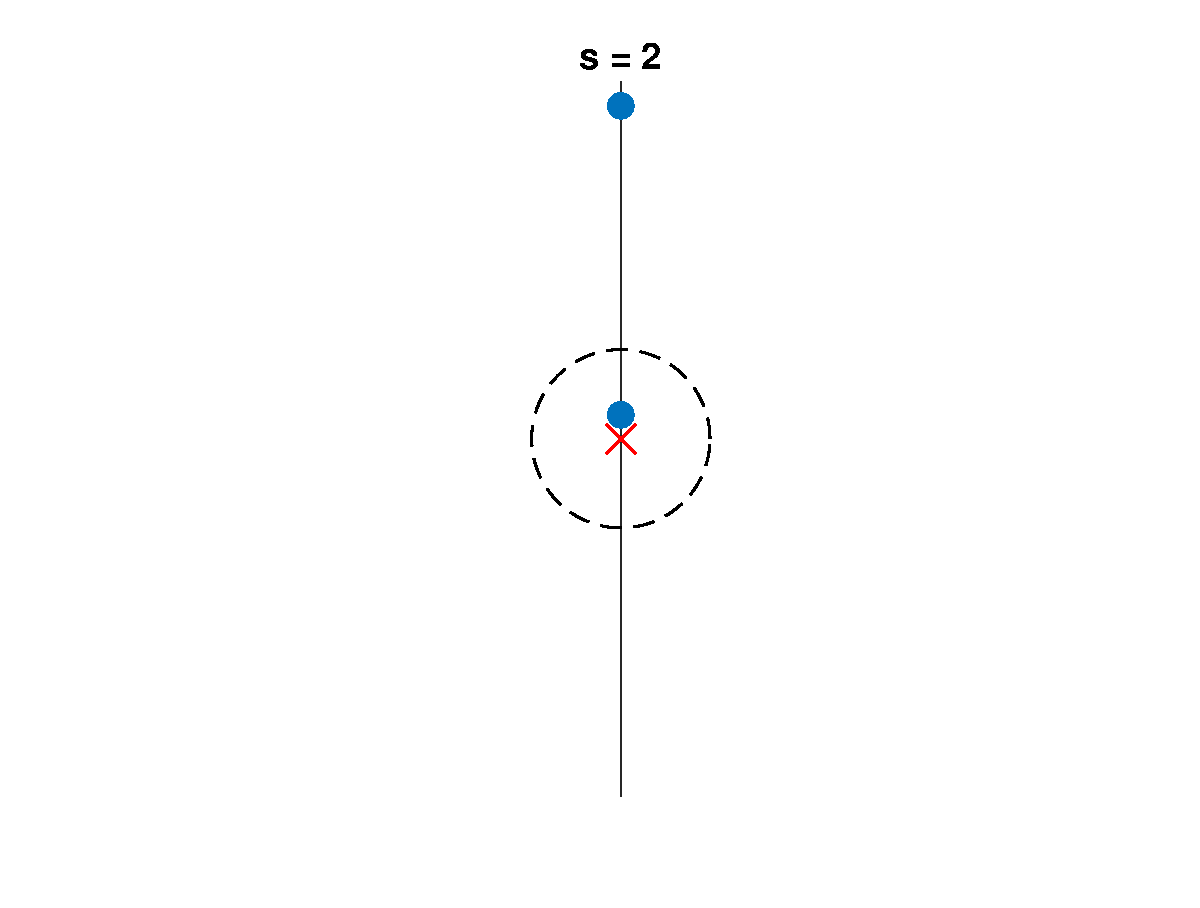
\includegraphics[width=5cm]{images/kreinbubbles/bubble2R} &
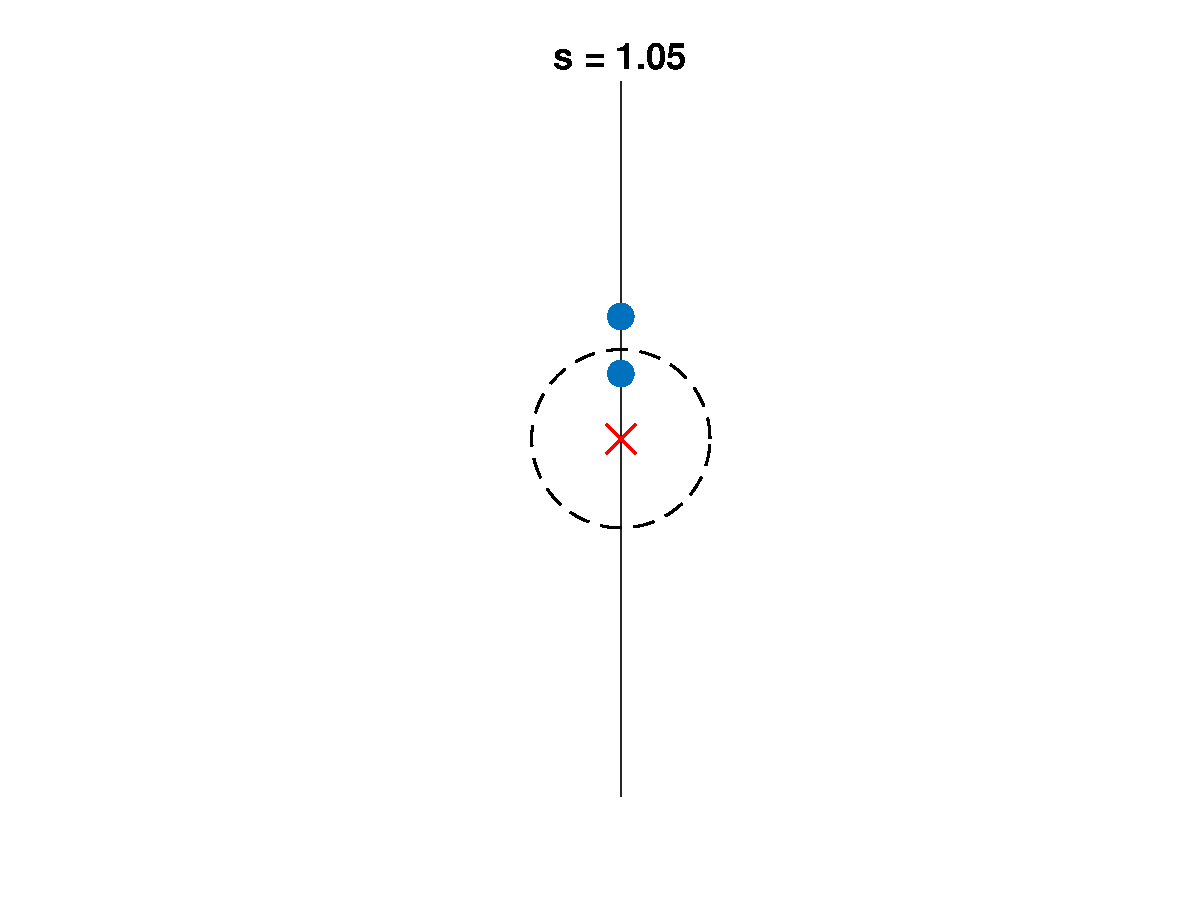
\includegraphics[width=5cm]{images/kreinbubbles/bubble105R} &
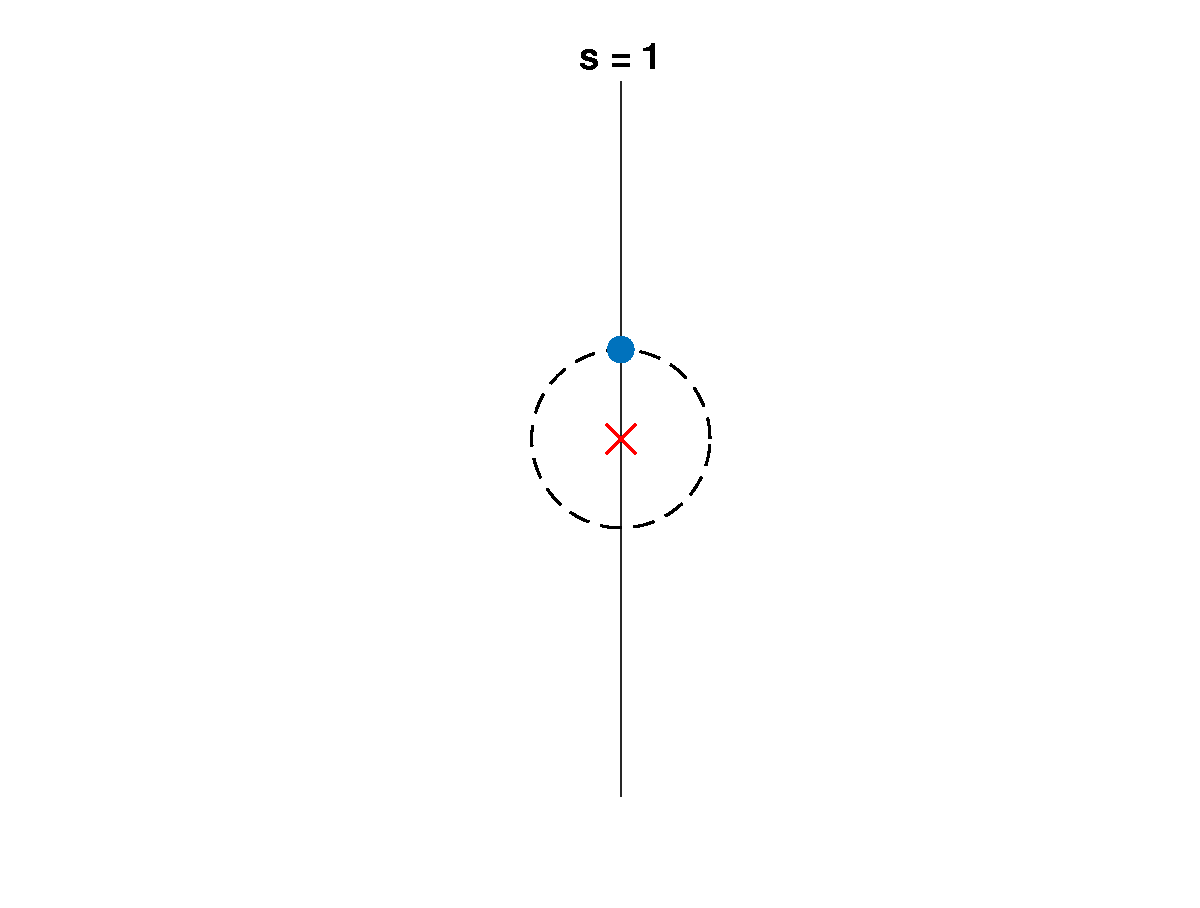
\includegraphics[width=5cm]{images/kreinbubbles/bubbleR} \\
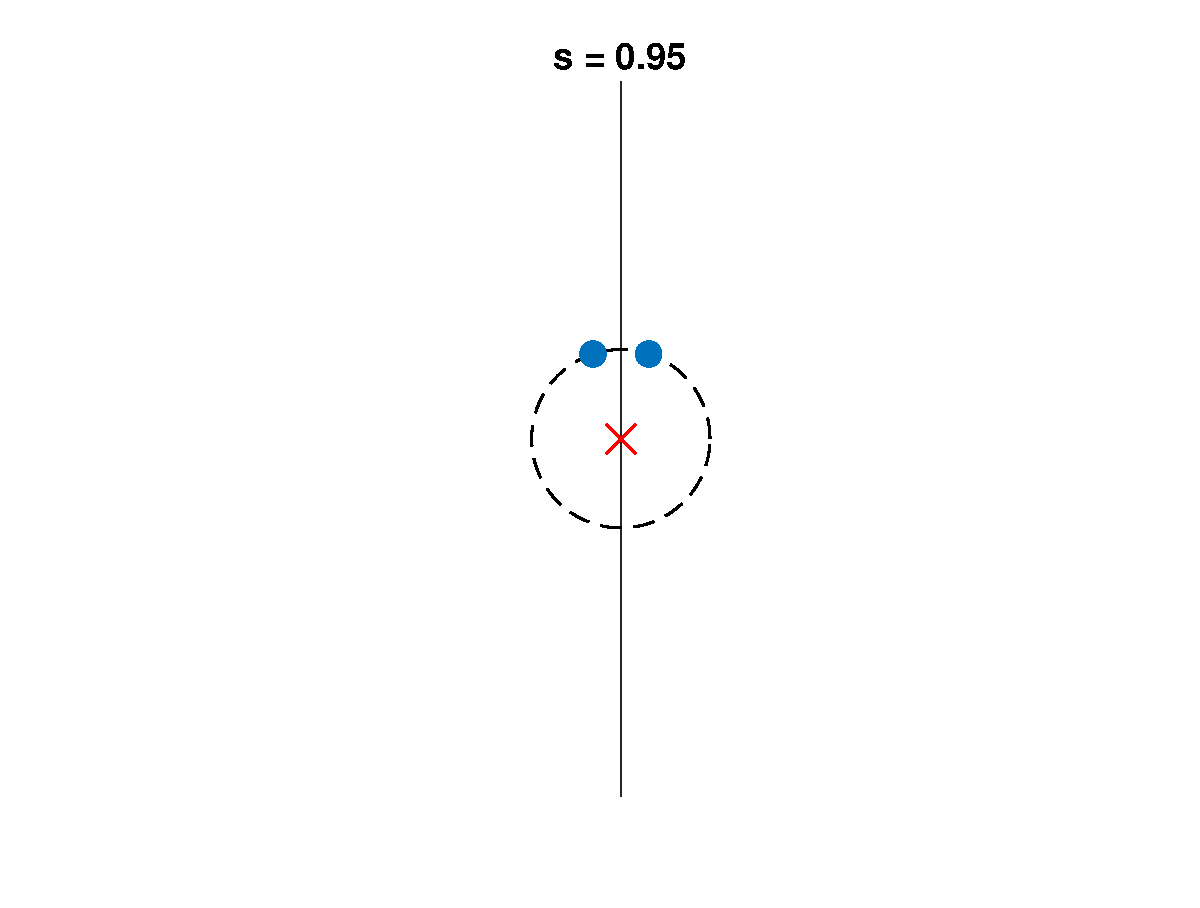
\includegraphics[width=5cm]{images/kreinbubbles/bubble095R} &
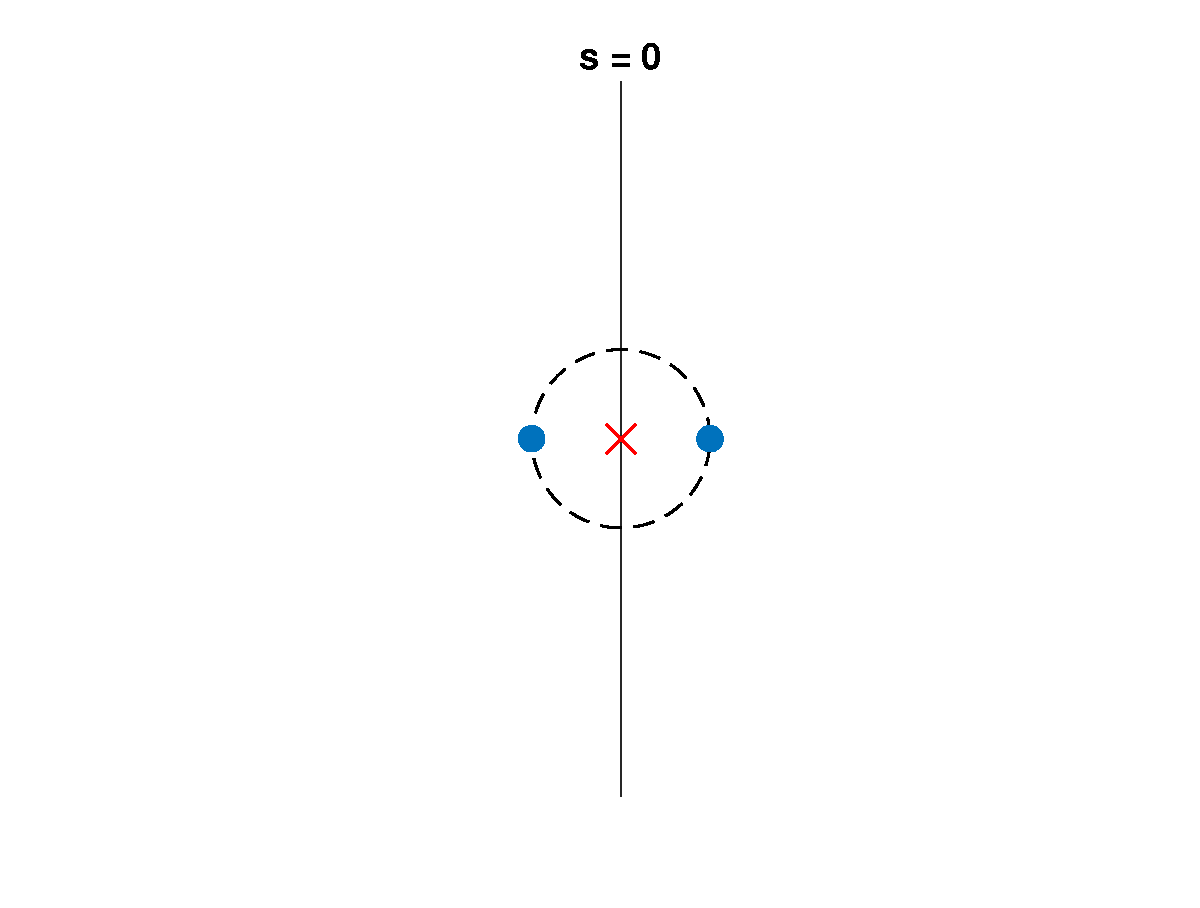
\includegraphics[width=5cm]{images/kreinbubbles/bubble0} &
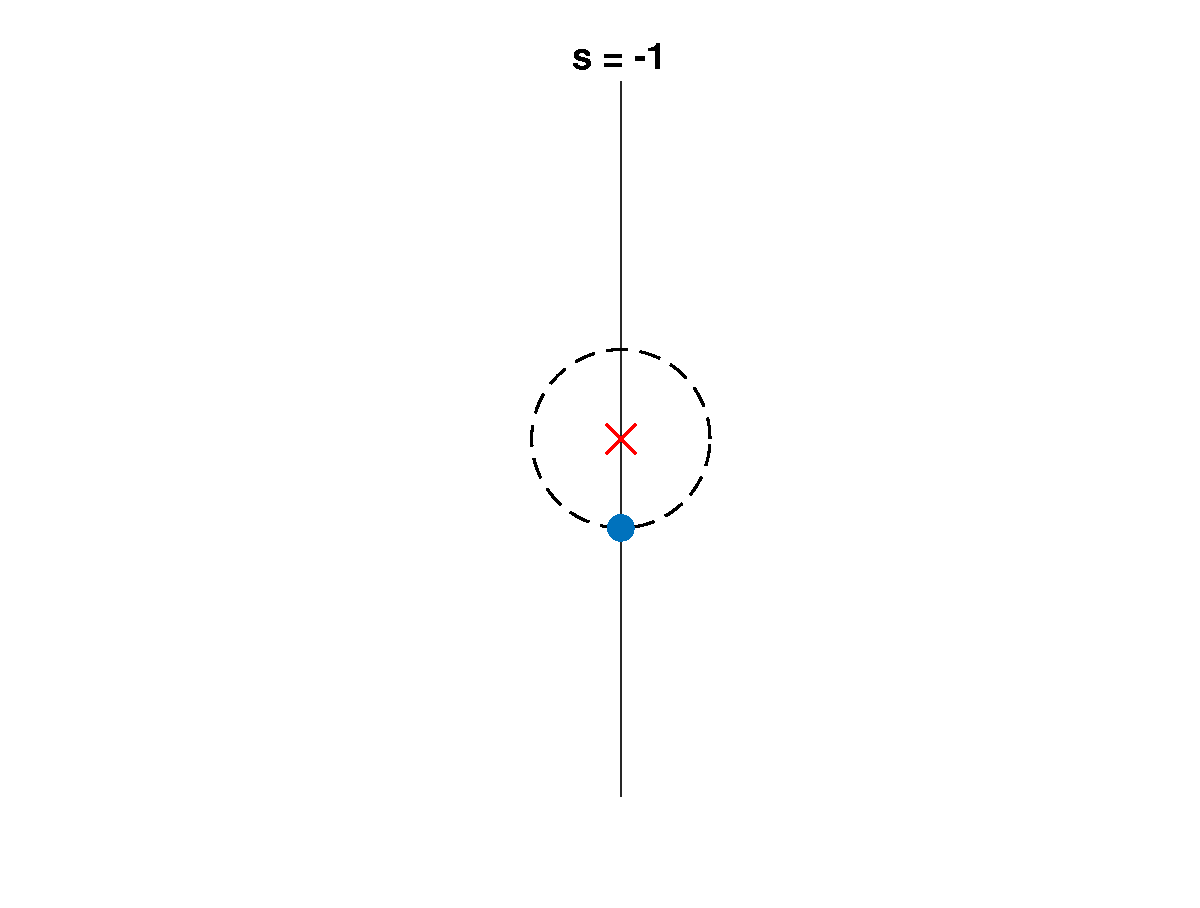
\includegraphics[width=5cm]{images/kreinbubbles/bubbleminusR}
\end{tabular}
\caption{Plot of the complex plane illustrating eigenvalue collision and Krein bubble as parameter $s$ is decreased. Blue dots are the pair of eigenvalues. Red cross is the point $\lambda_* i$. Vertical line is the imaginary axis. Black dotted circle is the circle of radius $\sqrt{R}$ around $\lambda_*$ }
\label{fig:kreinbubbles}
\end{center}
\end{figure}
We will call the instability bubble a Krein bubble, since it results from the collision of two imaginary eigenvalues with opposite Krein signatures. Inside the Krein bubble, the eigenvalues $\lambda_{1,2}$ are symmetric across the imaginary axis. Outside the Krein bubble, there is no such symmetry for $\lambda_{1,2}$; since $\lambda_{1,2}$ are purely imaginary, Hamiltonian symmetry tells that there exist eigenvalues $-\lambda_{1,2}$ which are below the real axis.

In the following theorem, we prove that these Krein bubbles occur. Since the bubbles are formed as $X$ is varied near $X^*$ we will parameterize both $X$ and the eigenvalues $\lambda_{1,2}$ by a single dimensionless parameter $s \in [-2, 2]$. THE ``h.o.t'' WILL BE SPECIFIED ONCE THE PROOF IS COMPLETE.

\begin{theorem}\label{theorem:kreinbubbles}
Let $\delta > 0$ be as in Theorem \ref{blockmatrixtheorem} [Theorem 5.4, the block matrix theorem]. Define
\begin{itemize}
\item $\lambda_* = \sqrt{\frac{2 a_0}{M}}$
\item $\lambda_k = c \frac{k \pi}{X}$, where $k$ is a positive integer such that $\lambda_k < \delta$.
\item $X_k^* = \frac{c k \pi}{\lambda_*}$
\item $R_0 = -\frac{4 p_1 k_0}{M}$ [OR SOMETHING CLOSE TO THIS], where $p_1$, $k_0$, and $M$ are defined in Theorem \ref{blockmatrixtheorem} [Theorem 5.4].
\item $R = \lambda_*^2 R_0 \frac{X_0}{X}$ 
\end{itemize}
Assume $R_0 > 0$. Then for sufficiently small $r$, the following is true. Let $s \in [-2, 2]$. For $X = X(s)$ close to $X_k^*$, there exists a pair of eigenvalues located at
\begin{align*}
\lambda_{1,2}(s) = \left( \lambda_* + s \sqrt{R} \right) i \pm \sqrt{R(1 - s^2)} + \text{``h.o.t.''}
\end{align*}
where
\[
X(s) = \frac{c k \pi}{s + \lambda_*}
\]
and $X(0) = X_k^*$. These eigenvalues have the following configuration.
\begin{itemize}
\item For $|s| < 1$, $\lambda_{1,2}(s)$ is symmetric across the imaginary axis, i.e. $\lambda_2(s) = -\overline{\lambda_1}(s)$. For $s = 0$, these are given by
\[
\lambda_{1,2}(s) = \lambda_* i \pm (\sqrt{R} + ``h.o.t.'')
\]
\item For $|s| \in (1, 2]$, $\lambda_{1,2}(s)$
are purely imaginary. For $s = 2$, one of $\lambda_{1,2}(s)$ is close to $\lambda_* i$.
\item At $s = \pm 1$, $\lambda_{1,2}(s)$ collide on the imaginary axis at 
\[
\lambda_{1,2}(s) = \lambda_* i \pm (\sqrt{R} + ``h.o.t.'')
\]
\end{itemize}
For $|s| \leq 1$, the eigenvalues $\lambda_{1,2}(s)$ are, to leading order, located on a circle of radius $\sqrt{R}$ about $\lambda_* i$ in the complex plane, where
\[
\sqrt{R} = \mathcal{O}\left( r^{3/4}\frac{X_0}{X} \right)
\]
\end{theorem}

\section{Determinant of block matrix}

In this section, we will compute the determinant of the block matrix from \cref{blockmatrixtheorem} for the periodic 2-pulse. This is a $4 \times 4$ matrix, and although the computation is tedious, it can be done with the aid of Mathematica. Before we can do that, we will prove the following bound which makes this computation significantly easier.

\begin{lemma}\label{lemma:expnubound}
Let $|\lambda| < \delta$. Then if either the conditions of Case 1 or Case 2 hold, we have the bound
\begin{equation}\label{expnubound}
\left|e^{\nu(\lambda)x}\right| \leq C \\
\end{equation}
for any $x$ with $|x| \leq X$, where the constant $C$ only depends on $\delta$.
\begin{proof}
Let $\lambda = a + bi$ with $|a| \leq C r^{1/2}/X^{1/2}$. Since $|\lambda| \leq \delta$, $|a|, |b| \leq \delta$ as well. Then from Lemma \ref{nulambdalemma},
\begin{align*}
\nu(\lambda) &= \frac{1}{c}\lambda + \mathcal{O}(\lambda^3) \\
&= \frac{a}{c} + i \frac{b}{c} + \mathcal{O}\left( a(a^2 + \delta^2) \right) + i \mathcal{O}\left( a(b^2 + \delta^2) \right)
\end{align*}
where both of the remainder terms are real. (We split the remainder up into real and imaginary parts). Thus 
\begin{align*}
\nu(\lambda)X &= \frac{a}{c}X + i \frac{b}{c}X + \mathcal{O}\left( a(a^2 + \delta^2) X\right) + i \mathcal{O}\left( a(b^2 + \delta^2) X\right)
\end{align*}
When we evaluate $|\exp{(\nu(\lambda)X)}|$, the two imaginary terms on the RHS do not contribute. For the other two terms, we consider Case 1 and Case 2 separately. For Case 1, $|a| \leq r^{1/2}$ and $r^{1/2}X < C$, thus
\begin{align*}
\left| \frac{a}{c}X + \mathcal{O}\left( a(a^2 + \delta^2) X \right) \right| &\leq C(1 + \mathcal{O}(|a|^2 + \delta^2)) \leq C.
\end{align*} 
For Case 2, $|a| \leq r^{1/2}/X^{1/2}$ and $r^{1/2}X^{1/2} < C$, thus
\begin{align*}
\left| \frac{a}{c}X + \mathcal{O}\left( a(a^2 + \delta^2) X \right) \right| &\leq C r^{1/2}X^{1/2}(1 + |a|^2 + \delta^2) \leq C r^{1/2}X^{1/2} (1 + \delta^2) \leq C
\end{align*} 
In both cases, the constant $C$ only depends on $\delta$, and so we have
\begin{align*}
|\exp{(\nu(\lambda)X)}| &\leq
\exp{ \left| \frac{a}{c}X + \mathcal{O}\left( a(a^2 + \delta^2) X \right) \right| } \leq C
\end{align*}
The same bound holds for $|x| \leq X$.
\end{proof}
\end{lemma}

Next, we compute the determinant of the block matrix in Theorem \ref{blockmatrixtheorem} for the periodic 2-pulse. Since this is a $4\times 4$ matrix with tons of remainder terms, our only hope is to do this with Mathematica.

\begin{lemma}\label{2blockmatrix}
For $|\lambda| < \delta$ with $|\Re \lambda| \leq C r^{1/2}X^{1/2}$, the determinant of the block matrix $B$ is 
\begin{equation}\label{2detBeq}
\begin{aligned}
\det &B(\lambda, r) = \left(-2 \lambda^2 M (2a + \lambda^2 M) +  \mathcal{O}( (r^{1/2} + |\lambda|)^5 )\right) \sinh(\nu(\lambda)X) \\
&+16 p_1 M \lambda^4 ( k_0\sinh(\nu(\lambda)X_0) + k_1 \sinh(\nu(\lambda)X_1) ) \cosh(\nu(\lambda)X)  \\
&+ \mathcal{O}( (r^{1/2} + |\lambda|)^6) 
\end{aligned}
\end{equation}
\begin{proof}
First, we write the block matrix $B$ as $B = B_1 + B_2$, where
\[
B_1 = \begin{pmatrix}
\begin{pmatrix}
e^{-\nu(\lambda)X_1} & -e^{\nu(\lambda)X_0} \\
-e^{\nu(\lambda)X_1} & e^{-\nu(\lambda)X_0} 
\end{pmatrix} &
2 \lambda \begin{pmatrix}
-e^{-\nu(\lambda)X_1} k_1 + e^{\nu(\lambda)X_0} k_0 & e^{-\nu(\lambda)X_1} k_1 - e^{\nu(\lambda)X_0} k_0 \\ e^{-\nu(\lambda)X_0} k_0 - e^{\nu(\lambda)X_1} k_1 & -e^{-\nu(\lambda)X_0} k_0 + e^{\nu(\lambda)X_1} k_1
\end{pmatrix} \\
p_1 \lambda
\begin{pmatrix}
e^{-\nu(\lambda)X_1} & e^{\nu(\lambda)X_0} \\
e^{\nu(\lambda)X_1} & e^{-\nu(\lambda)X_0} 
\end{pmatrix} &
\begin{pmatrix}
-a - \lambda^2 M & a \\
a & -a - \lambda^2 M
\end{pmatrix}
\end{pmatrix}
\]
and $B_2$ is the block matrix 
\[
B_2 = \begin{pmatrix}
G_1 & G_2 \\ G_3 & G_4
\end{pmatrix}
\]
By our choice of $\lambda$, it follows from \cref{lemma:expnubound} that all the terms of the form $e^{\pm \nu(\lambda)X_j}$ are bounded by a constant. Thus the remainder matrices $G_i$ have bounds
\begin{equation}\label{Gimatrixbounds}
\begin{aligned}
|G_1| &\leq C |\lambda| (|\lambda| + r^{1/2} )\\
|G_2| &\leq C |\lambda| (|\lambda| + r^{1/2} )^2 \\
|G_3| &\leq C (|\lambda| + r^{1/2} )^2 \\
|G_4| &\leq C (|\lambda| + r^{1/2} )^3 \\
\end{aligned}
\end{equation}
We use Mathematica to evaluate the determinant. Briefly, we write the matrices $G_j$ as
\[
G_j = \begin{pmatrix}t^j_1 & t^j_2 \\ t^j_3 & t^j_4 \end{pmatrix}
\]
where the the coefficients $t^j_k$ have bounds given by \cref{Gimatrixbounds}. We then use Mathematica to expand the determinant, and we track each of the $t^j_k$. Doing all of this, we have
\begin{equation}\label{2detB1}
\begin{aligned}
\det &B(\lambda, r) = \sinh(\nu(\lambda)X)\left(-2 \lambda^2 M (2a + \lambda^2 M) +  \mathcal{O}( (r^{1/2} + |\lambda|)^5 )\right) \\
&+4\lambda^4 p_1 k_0 M \left( \sinh(\nu(\lambda)(2 X_0 + X_1)) - 3 \sinh(\nu(\lambda)X_1)  \right) \\
&+4\lambda^4 p_1 k_1 M \left( \sinh(\nu(\lambda)(2 X_1 + X_0)) - 3 \sinh(\nu(\lambda)X_0)  \right) \\
&+ \mathcal{O}( (r^{1/2} + |\lambda|)^6) 
\end{aligned}
\end{equation}
Using standard hyperbolic trigonometric identities, we can show that 
\begin{align*}
\sinh(2 x + y) - 3 \sinh(y) &= 4 \cosh(x + y)\sinh(x) 
-2 \sinh(x+y)\cosh(x) 
\end{align*}
Using this with the second line of \cref{2detB1}, 
\begin{align*}
\lambda^4 &k_0 \left( \sinh(\nu(\lambda)(2 X_0 + X_1)) - 3 \sinh(\nu(\lambda)X_1)  \right) \\
&= 4 \lambda^4 k_0 \cosh(\nu(\lambda)X)\sinh(\nu(\lambda)X_0) - 3 \lambda^4 k_0 \sinh(\nu(\lambda)X)\cosh(\nu(\lambda)X_0) \\
&= 4 \lambda^4 k_0 \cosh(\nu(\lambda)X)\sinh(\nu(\lambda)X_0) + \sinh(\nu(\lambda)X)(\mathcal{O}(r^{1/2}|\lambda|^4))
\end{align*}
since $k_0 = \mathcal{O}(r^{1/2})$ and $|\cosh(\nu(\lambda)X_0)|\leq C$ by Lemma \ref{lemma:expnubound}. Doing the same thing for the third line of \cref{2detB1}, we have
\begin{equation*}
\begin{aligned}
\det &B(\lambda, r) = \left(-2 \lambda^2 M (2a + \lambda^2 M) +  \mathcal{O}( (r^{1/2} + |\lambda|)^5 )\right) \sinh(\nu(\lambda)X) \\
&+16 p_1 M \lambda^4 ( k_0\sinh(\nu(\lambda)X_0) + k_1 \sinh(\nu(\lambda)X_1) ) \cosh(\nu(\lambda)X)  \\
&+ \mathcal{O}( (r^{1/2} + |\lambda|)^6) 
\end{aligned}
\end{equation*}
\end{proof}
\end{lemma}

We now have an equation we can solve to find the eigenvalues $\lambda$. However, this equation involves both $\lambda$ and $\nu(\lambda)$, which is annoying. We will simplify the problem by making a change of variables. Since $\nu'(0) = 1/c$ and $\nu(0) = 0$, $\nu(\lambda)$ is invertible near 0. If necessary, decrease $\delta$ so that $\nu(\lambda)$ is invertible for $|\lambda| < \delta$. Let $\lambda = \nu^{-1}(\mu)$. Expanding in Taylor series about $\mu = 0$, we have
\[
\nu^{-1}(\mu) = c \mu + \mathcal{O}(\mu^3)
\]
Substituting this into \cref{2detBeq} and simplifying, 
\begin{equation}\label{2detBeqmu}
\begin{aligned}
\det &B(\mu, r) = \left(-2 c^2 \mu^2 M (2a + c^2 \mu^2 M) +  \mathcal{O}( (r^{1/2} + |\mu|)^5 )\right) \sinh(\mu X) \\
&+16 p_1 M \mu^4 ( k_0\sinh(\mu X_0) + k_1 \sinh(\mu X_1) ) \cosh(\mu X)  \\
&+ \mathcal{O}( (r^{1/2} + |\mu|)^6) 
\end{aligned}
\end{equation}
To find the eigenvalues, we will find the zeros of \cref{2detBeqmu}. We will do this for several specific cases.

\section{Computation of coefficients $a_j$}

Next, we compute the coefficients $a_j$ of the matrix $A$ in lower right block of the block matrix equation.

\begin{lemma}

\begin{proof}
Taking the derivative of $\langle \Psi(x), Q(-x) \rangle$, we have
\begin{align*}
\frac{d}{dx} \langle \Psi(x), Q(-x) \rangle
&= \langle \Psi'(x), Q(-x) \rangle - \langle \Psi(x), Q'(-x) \rangle
\end{align*}
Extract the last components of $\Psi(x)$ and $Q(x)$ by letting $\Psi(x) = (\tilde{\Psi}(x), q(x))$ and $Q(x) = (\tilde{Q}(x), 0)$. For the first inner product, since $\tilde{\Psi}(x)$ solves \cref{adjvareq1},
\begin{align*}
\langle \Psi'(x), Q(-x) \rangle &= \langle \tilde{\Psi}'(x), \tilde{Q}(-x) \rangle \\
&= \langle -DF(Q(x))^* \tilde{\Psi}'(x), \tilde{Q}(-x) \rangle \\
&= - \langle \tilde{\Psi}(x), DF(Q(x)) \tilde{Q}(-x) \rangle 
\end{align*}
\end{proof}
\end{lemma}

\begin{lemma}\label{lemma:ajparam}
For the coefficients $a_j$ in the block matrix equation, 
\begin{equation}\label{ajparam}
a_j = s_0 e^{\alpha \phi/\beta} r b_j \left( \beta \cos\left(-\rho \log b_j \right) - \alpha \sin \left(-\rho \log b_j \right) \right) + \mathcal{O}(r^{1+\gamma/2\alpha})
\end{equation}

\begin{proof}
From \cite[Lemma 6.1]{Sandstede1998},
\begin{align*}\label{IPpsiQprime}
\langle \Psi(-x), Q'(x) \rangle
&= s_0 e^{-2 \alpha x}\left( \beta \cos(2 \beta x + \phi) - \alpha \sin(2 \beta x + \phi)\right) + \mathcal{O}(e^{-(2 \alpha + \gamma) x}
\end{align*}
where $s_0 > 0$ and $\gamma$ are the same as in Lemma \ref{IPform}. Thus we have
\begin{align*}
a_j &= \langle \Psi(-X_j), Q'(X_j) \rangle \\
&= s_0 e^{-2 \alpha X_j}\left( \beta \cos(2 \beta X_j + \phi) - \alpha \sin(2 \beta X_j + \phi)\right) + \mathcal{O}(e^{-(2 \alpha + \gamma) X_j}) \\
&= s_0 e^{\alpha \phi/\beta} r b_j \left( \beta \cos\left( -\frac{\beta}{\alpha} \log(b_j r) \right) - \alpha \sin \left( -\frac{\beta}{\alpha} \log(b_j r) \right) \right) + \mathcal{O}(r^{1+\gamma/2\alpha} b_j^{1 + \gamma/2\alpha}) \\
&= s_0 e^{\alpha \phi/\beta} r b_j \left( \beta \cos\left( -\rho \log(b_j r) \right) - \alpha \sin \left( -\rho \log(b_j r) \right) \right) + \mathcal{O}(r^{1+\gamma/2\alpha})
\end{align*}
since $b_j \in (0, 1]$. Since $r \in \mathcal{R}$, $r = \exp\left(-\frac{2 m \pi}{\rho}\right)$ for some nonnegative integer $m$, this becomes 
\begin{align*}
a_j &= s_0 e^{\alpha \phi/\beta} r b_j \left( \beta \cos\left( 2 m \pi -\rho \log b_j \right) - \alpha \sin \left( 2 m \pi -\rho \log b_j \right) \right) + \mathcal{O}(r^{1+\gamma/2\alpha}) \\
&= s_0 e^{\alpha \phi/\beta} r b_j \left( \beta \cos\left(-\rho \log b_j \right) - \alpha \sin \left(-\rho \log b_j \right) \right) + \mathcal{O}(r^{1+\gamma/2\alpha})
\end{align*}
\end{proof}
\end{lemma}

\section{Essential spectrum eigenvalues}

In this section, we will look for the essential spectrum eigenvalues. We will only do this for Case 1. In terms of $\mu$, we expect to find the essential spectrum eigenvalues near $\pm m \pi i/X$ for integer $k$. Let $r_0$ be as above, and for $r = r_0$, let $M$ be the largest integer such that $\left| \frac{M \pi}{X} \right| < \delta$. Let $m$ be a nonzero integer with $|m| \leq M$, and let
\[
\mu_m = \frac{m \pi i}{X} + \frac{h}{X}
\]
Expanding the $\sinh(\mu_m X)$ and $\cosh(\mu_m X)$ terms in \cref{2detBeqmu} about $m \pi/X$, we have
\begin{align*}
\sinh(\mu_m X) &= (-1)^m h + \mathcal{O}(h^3) \\
\cosh(\mu_m X) &= (-1)^m + \mathcal{O}(h^2) \\
\end{align*}
By \cref{lemma:expnubound}, the $\sinh(\mu_m X_j)$ terms in \cref{2detBeqmu} are bounded by a constant. The $k_j$ terms are $\mathcal{O}(r^{1/2})$. By the assumptions in Case 1, $|\mu_m| \geq C r^{1/2}$. Substituting these into \cref{2detBeqmu}, we have 
\begin{equation}\label{Bess1}
\begin{aligned}
\det &B(h, r) = \left(-2 c^2 M  \mu_m^2 \left( 2a + c^2 M \mu_m \right)^2 + \mathcal{O}( |\mu_m|)^5 \right) \left( (-1)^m h + \mathcal{O}(h^3) \right) \\
&+ \mu_m^4 \left( (-1)^m + \mathcal{O}(h^2)\right)\mathcal{O}(r^{1/2}) + \mathcal{O}\left( |\mu_m| \right)^6 \\
&= \left(-2 c^2 M  \mu_m^2 \left( 2a + c^2 M \mu_m \right)^2 + \mathcal{O}( |\mu_m|)^5 \right) \left( (-1)^m h + \mathcal{O}(h^3) \right) + \mathcal{O}\left( |\mu_m|^4(r^{1/2} + |\mu_m|) \right)
\end{aligned}
\end{equation}
We want to solve $\det B(\mu, r) = 0$. To simplify, let $\mu_* = \sqrt{-\frac{2a}{M c^2}}$. Dividing by $(-1)^m$, $M c^2$, and the constants out front, we want to solve 
\begin{equation}\label{Bess2}
\begin{aligned}
\left(\mu_m^2 (\mu_m - \lambda_*)(\mu_m + \lambda_*) + \mathcal{O}( |\mu_m|)^5 \right) \left( h + \mathcal{O}(h^3) \right) + \mathcal{O}\left( |\mu_m|^4(r^{1/2} + |\mu_m|) \right) = 0
\end{aligned}
\end{equation}
Since $\mu_m \neq 0$, divide by $\mu_m^2$ to get
\begin{equation}\label{Bess3}
\begin{aligned}
\left((\mu_m - \lambda_*)(\mu_m + \lambda_*) + \mathcal{O}( |\mu_m|)^3 \right) \left( h + \mathcal{O}(h^3) \right) + \mathcal{O}\left( |\mu_m|^2(r^{1/2} + |\mu_m|) \right) = 0
\end{aligned}
\end{equation}
Finally, multiply by $X^2$ and substitute for $\mu_m$. Since $m \leq M$, simplify the remainder terms to get $F_m(h, r) = 0$, where
\begin{equation}\label{Bess4}
\begin{aligned}
F_m(h, r) &= (m \pi i + h - \lambda_* X)(m \pi i + h + \lambda_* X) \left( h + \mathcal{O}(h^3) \right) + \mathcal{O}\left( r^{1/2} + \frac{1}{X} \right)
\end{aligned}
\end{equation}
Since $X = \mathcal{O}(1/\log|r|)$, $F(0,0) = 0$. Since $\lambda_* = \mathcal{O}(r^{1/2})$, $\lambda_* X \rightarrow 0$ as $r \rightarrow 0$. Thus we have
\[
\partial_h F(0,0) = -m^2 \pi^2
\]
For all $m$ between 1 and $M$, $|\partial_h F(0,0)| \geq \pi^2 > 0$. Thus we can use the implicit function theorem to solve for $h$ in terms of $r$ near $h = 0$. Specifically, there exists $r_1^m \leq r_0$ and a unique smooth function $h_m(r)$ with $h_m(0) = 0$ such that for all $r \leq r_1^m$, $G(h_m(r),r) = 0$. Expanding $h_m$ in a Taylor series about $r = 0$, we have for all $|m| \leq M$,
\[
h_m(r) = \mathcal{O}\left( r^{1/2} + \frac{1}{X} \right)
\]
Do this for all $|m| \leq M$, and let $r_1 = \min\{ r_1^m \}$. Undoing the scaling, for all $r \leq r_1$ and for all nonzero integers $m$ with $|m| \leq M$, there are essential spectrum eigenvalues located at
\[
\mu_m = \frac{m \pi i}{X} + \mathcal{O}\left( \frac{1}{X}\left( r^{1/2} + \frac{1}{X} \right) \right)
\]
Changing variables back to $\lambda$, these are located at
\[
\lambda_m = \frac{m \pi i}{X}\left[1 + \mathcal{O}\left( \frac{1}{X}\left( r^{1/2} + \frac{1}{X} \right) \right) \right] + \mathcal{O}\left( \frac{1}{X}\left( r^{1/2} + \frac{1}{X} \right) \right)
\]
By Hamiltonian symmetry, eigenvalues must come in quartets. Thus $\lambda_m$ is pure imaginary and $\lambda_{-m} = \lambda_m$. We conclude that the nonzero essential spectrum eigenvalues are given by $\lambda = \pm \lambda_m^{\text{ess}}$, where
\[
\lambda_m^{\text{ess}} = \frac{m \pi i}{X}\left[1 + \mathcal{O}\left( \frac{1}{X}\left( r^{1/2} + \frac{1}{X} \right) \right) \right] + \mathcal{O}\left( \frac{1}{X}\left( r^{1/2} + \frac{1}{X} \right) \right)
\]
is pure imaginary. This proves \cref{theorem:2peigscase1} part (ii).

\section{Interaction eigenvalues}

In this section, we will set up the estimates we need for parts (i) and (iii) of \cref{theorem:2peigscase1}. In both cases, we are looking for eigenvalue $\lambda$ of order $r^{1/2}$. Thus \cref{2detBeqmu} simplifies to
\begin{equation}\label{2detBint1}
\begin{aligned}
\det &B(\mu, r) = \left(-2 c^2 \mu^2 M (2a + c^2 \mu^2 M) +  \mathcal{O}( r^{5/2} )\right) \sinh(\mu X) \\
&+16 p_1 M \mu^4 ( k_0\sinh(\mu X_0) + k_1 \sinh(\mu X_1) ) \cosh(\mu X) + \mathcal{O}( r^3 ) 
\end{aligned}
\end{equation}
For Case 1, $\lambda X \leq c/2$, thus $\mu X \leq 1/2$. We expand the $\sinh$ and $\cosh$ terms in a Taylor series about 0 to get
\begin{align*}
\sinh(\mu X) &= \mu X + \mathcal{O}\left(\mu X \right)^3 \\
\cosh(\mu X) &= 1 + \mathcal{O}\left(\mu X)^2 \\
\sinh(\mu X_j) &= \mu X_j + \mathcal{O}\left(\mu X_j \right)^3
\end{align*}
Substituting these and simplifying, we obtain 
\begin{equation}\label{2detBint2}
\begin{aligned}
\det &B(\mu, r) = \left(-2 c^2 \mu^2 M (2a + c^2 \mu^2 M) +  \mathcal{O}( r^{5/2} )\right) \left(\mu X + \mathcal{O}\left(\mu X \right)^3 \right) \\
&+16 p_1 M \mu^4 \left( k_0\left( \mu X_0 + \mathcal{O}\left(\mu X_0 \right)^3\right) + k_1\left( \mu X_1 + \mathcal{O}\left(\mu X_1 \right)^3\right) \right) \left( 1 + \mathcal{O}\left(\mu X)^2\right) \\
&+ \mathcal{O}( r^3 ) 
\end{aligned}
\end{equation}
Since $k_j$ terms are $\mathcal{O}(r^{1/2})$, this simplifies to 
\begin{equation}\label{2detBint2}
\begin{aligned}
\det &B(\mu, r) = -2 c^2 \mu^2 M (2a + c^2 \mu^2 M)\left( \mu X + \mathcal{O}\left(\mu X \right)^3 \right) 
+ \mathcal{O}( r^3 X ) 
\end{aligned}
\end{equation}
We wish to solve the equation $\det B(\mu, r) = 0$. Next, we scale out the scaling parameter $r$ from the eigenvalues. Let $\mu = r^{1/2}\tilde{\mu}$ and $a = r \tilde{a}(r) = r (\tilde{a}_1(r) + \tilde{a}_2(r))$. From Lemma \ref{lemma:ajparam}, 
\begin{align}\label{tildea1}
\tilde{a}_j(r) &= s_0 e^{\alpha \phi/\beta} b_j(r) \left( \beta \cos\left(-\rho \log b_j(r) \right) - \alpha \sin \left(-\rho \log b_j(r) \right) \right) + \mathcal{O}(r^{1+\gamma/2\alpha})
\end{align}
Making this substitution and dividing by $r^{5/2}$ and the constants out front, we want to solve
\begin{equation}\label{2detBint4}
\begin{aligned}
\tilde{\mu}^2 (2\tilde{a}(r) + c^2 \tilde{\mu}^2 M)\left( \tilde{\mu} X + \mathcal{O}(r X^3)\right) + \mathcal{O}( r^{1/2} X ) = 0
\end{aligned}
\end{equation}
Let $\tilde{\mu}_*(r) = \sqrt{-\frac{2\tilde{a}(r)}{M c^2}}$. Dividing by $X$ and $c^2 M$ and simplifying, we wish to solve $G(\tilde{\mu},r) = 0$, where
\begin{equation}\label{2detBint4}
\begin{aligned}
G(\tilde{\mu},r) = \tilde{\mu}^2 (\tilde{\mu} - \tilde{\mu}_*(r))(\tilde{\mu} + \tilde{\mu}_*(r))\left( \tilde{\mu} + \mathcal{O}(r X^2)\right) + \mathcal{O}( r^{1/2} ) = 0
\end{aligned}
\end{equation}
We expect to have interaction eigenvalues near $\tilde{\mu} = \pm \tilde{\mu}_*(0)$. Taking the derivative with respect to $\tilde{\mu}$ at $\pm \tilde{\mu}_*$, we have
\[
\partial_{\tilde{\mu}} G(\pm \tilde{\mu}_*,0) = 2 \tilde{\mu}_*(0)^4 
\]
which is 0 if and only if $\tilde{a}(0) = 0$. We will now prove a result giving a criterion for when $\tilde{a}(0) = 0$.

\begin{lemma}\label{lemma:tildea0zero}
$\tilde{a}_0 = 0$ if and only if the 2-pulse $Q_2(x)$ is parameterized by $b_0(0) = b_1(0) = p_k^*$, where $p_k^*$ is one of the pitchfork bifurcation points in the limiting case where $r = 0$.
\begin{proof}
For convenience, let $b_j = b_j(0)$. From \cref{tildea1},
\begin{align*}
\tilde{a}_j(0) &= s_0 e^{\alpha \phi/\beta} b_j \left( \beta \cos\left(-\rho \log b_j \right) - \alpha \sin \left(-\rho \log b_j \right) \right)
\end{align*}
thus we have
\begin{align}\label{tildea0}
\tilde{a}(0) &= s_0 e^{\alpha \phi/\beta}\left[ b_0 \left( \beta \cos\left(-\rho \log b_0 \right) - \alpha \sin \left(-\rho \log b_0 \right)  + b_1 \left( \beta \cos\left(-\rho \log b_1 \right) - \alpha \sin \left(-\rho \log b_1 \right) \right]
\end{align}
Recall from the construction of the periodic 2-pulse that
\begin{equation}\label{b0b1relation}
b_0 \sin \left(-\rho \log b_0) = b_1 \sin \left(-\rho \log b_1)
\end{equation}
BY A TEDIOUS COMPUTATION WHICH IS NOT YET DONE BUT VERY STRONGLY SUGGESTED BY NUMERICS, the only solution to $\tilde{a}(0) = 0$ which satisfies \cref{b0b1relation} is given by 
\[
b_0 = b_1 = p_k^*
\]
for integer $k$, where $p_k^*$ is one of the pitchfork bifurcation points in the zero set of $H(b_0, b_1)$ from Lemma \ref{pitchforkH}.
\end{proof}
\end{lemma}

Since the pitchfork bifurcation points only happen along the diagonal, we will consider the cases of asymmetric and symmetric periodic 2-pulses separately.

\subsection{Asymmetric periodic 2-pulses}

In the asymmetric case, if $X_1 > X_0$, then $b_0(0) \neq b_1(0)$. By \cref{lemma:tildea0zero}, $\tilde{a}_0 \neq 0$, thus $\tilde{\mu}_*(0) \neq 0$. Thus we can use the implicit function theorem to solve \cref{2detBint4} for $\tilde{\mu}$ in terms of $r$ near $\pm \tilde{\mu}_*(0)$. Specifically, there exists $r_1 \leq r_0$ and unique smooth functions $\tilde{\mu}^\pm(r)$ with $\tilde{\mu}^\pm(0) = \pm \tilde{\mu}_*(0)$ such that for all $r \leq r_1^m$, $G(\tilde{\mu}^\pm(r), r) = 0$. Expanding $\tilde{\mu}^\pm(r)$ in a Taylor series about $r = 0$, we have
for all $r \leq r_1$,
\[
\tilde{\mu}^\pm(r) = \pm \tilde{\mu}_*(0) + \mathcal{O}( r^{1/2} )
\]
Undoing the scaling, for all $r \leq r_1$, there are interaction eigenvalues located at
\begin{align*}
\mu^\pm(r) = \sqrt{-\frac{2 a(0)}{M c^2}} + \mathcal{O}( r^{1/2} )
\end{align*}
Changing variables back to $\lambda$, these are located at
\begin{align*}
\lambda^\pm(r) = \sqrt{-\frac{2 a(0)}{M}} + \mathcal{O}( r^{1/2} )
\end{align*}
By Hamiltonian symmetry, eigenvalues must come in quartets. Thus $\lambda^-(r) = -\lambda^+(r)$, and is either real or pure imaginary. We conclude that there is a pair of interaction eigenvalues which are either real or pure imaginary and are given by
\[
\lambda_m^{\text{ess}} = \frac{m \pi i}{X}\left[1 + \mathcal{O}\left( \frac{1}{X}\left( r^{1/2} + \frac{1}{X} \right) \right) \right] + \mathcal{O}\left( \frac{1}{X}\left( r^{1/2} + \frac{1}{X} \right) \right)
\]
This proves \cref{theorem:2peigscase1} part (i).
\[
\lambda^{\text{int}} = \pm \left( \sqrt{-\frac{2 a(0)}{M}} + \mathcal{O}( r^{1/2} ) \right)
\]

\subsection{Symmetric periodic 2-pulses}

In this section, we will look at the interaction eigenvalues of the symmetric periodic 2-pulse. For this case, $X_1 = X_0$, $X = 2 X_0$, $k_0 = k_1$, and $a = 2 a_0$. Let
\[
\mu_* = \sqrt{-\frac{4a_0}{M c^2}}
\]
Thus we have
\begin{equation}\label{Bsymmetric1}
\begin{aligned}
\det &B(\mu, r) = \left(-2 c^2 \mu^2 M (4a_0 + c^2 \mu^2 M) +  \mathcal{O}( (r^{1/2} + |\mu|)^5 )\right) \sinh(2 \mu X_0) \\
&+32 p_1 M \mu^4 k_0\sinh(\mu X_0) \cosh(2 \mu X_0) + \mathcal{O}( (r^{1/2} + |\mu|)^6) 
\end{aligned}
\end{equation}
Since $a = \mathcal{O}(r)$, $\mu = \mathcal{O}(r^{1/2})$. We are looking for $\mu$ close to $\lambda_*$. Since $X_0 = \mathcal{O}(\log|r|)$, choose $r$ sufficiently small so that $\mu X_0 < 1/2$. Then we can expand the $\sinh$ and $\cosh$ terms in a Taylor series about 0 to get
\begin{align*}
\sinh(2\mu X_0) &= 2 \mu X_0 + \mathcal{O}\left(\mu X_0 \right)^3 \\
\cosh(2\mu X_0) &= 1 + \mathcal{O}\left(\mu X_0 \right)^2
\end{align*}
Substituting these, we have
\begin{equation}\label{Bsymmetric2}
\begin{aligned}
\det &B(\mu, r) = \left(-2 c^2 \mu^2 M (4a_0 + c^2 \mu^2 M) +  \mathcal{O}( (r^{1/2} + |\mu|)^5 )\right) \left( 2 \mu X_0 + \mathcal{O}\left(\mu X_0 \right)^3 \right) \\
&+32 p_1 M \mu^4 k_0 \left( 2 \mu X_0 + \mathcal{O}\left(\mu X_0 \right)^3 \right) \left( 1 + \mathcal{O}\left(\mu X_0 \right)^2 \right) + \mathcal{O}( (r^{1/2} + |\mu|)^6) 
\end{aligned}
\end{equation}
Using $\mu = \mathcal{O}(r^{1/2})$, $k_0 = \mathcal{O}(r^{1/2})$, and dividing by the constants out front, we obtain the equation
\begin{equation*}
\begin{aligned}
G(\mu, r) = \mu^2 (4a_0 + c^2 \mu^2 M) \mu X_0 + \mathcal{O}( r^3 X_0 ) 
\end{aligned}
\end{equation*}
Dividing by $c^2 M$ and $X_0$, and letting
\begin{equation}
\mu_* = \sqrt{- \frac{4 a_0}{c^2 M}}
\end{equation}
this becomes
\begin{equation*}
\begin{aligned}
G(\mu, r) = \mu^3 (\mu - \mu_*)(\mu + \mu_*) + \mathcal{O}( r^3 ) 
\end{aligned}
\end{equation*}
Rescale the system by taking $\mu = r^{1/2} \tilde{\mu}$ and $\mu_* = r^{1/2} \tilde{\mu_*}$. Substituting these and dividing by $r^{5/2}$, we have
\begin{equation*}
\begin{aligned}
G(\tilde{\mu}, r) = \tilde{\mu}^3 (\tilde{\mu} - \tilde{\mu}_*)(\tilde{\mu} + \tilde{\mu}_*) + \mathcal{O}( r^{1/2} ) 
\end{aligned}
\end{equation*}
For $r = 0$, this has a triple zero at $\tilde{\mu} = 0$, which corresponds to the three kernel eigenfunctions. The interaction eigenvalues will occur near $\mu = \pm \tilde{\mu}$. At $\mu = \pm \pm \tilde{\mu}$, 
\[
\partial_{\tilde{\mu}}G(\pm \tilde{\mu}_*, 0) = 2 \tilde{\mu}_*^4
\]
Thus as long as $\tilde{\mu}_* \neq 0$, we can use the IFT. Since $\tilde{\mu}_* = 0$ if and only if $a_0 = 0$, we need to figure out when $a_0 = 0$. For the symmetric periodic 2-pulse, the baseline length parameters are $b_0^0 = b_0^0$, which are either $1$ or $e^{-\frac{1}{\rho} \pi}$. Thus for the length parameters, we have
\[
b_0^*(m, \theta) = b_1^*(m, \theta) = e^{-\frac{1}{\rho}(m \pi - \theta) }
\]
where either $m = 0$ or $m = 1$. Substituting these into the expression \cref{ajparam} from \cref{lemma:ajparam}, 
\begin{align*}
a_0 &= s_0 e^{\alpha \phi/\beta} r e^{-\frac{1}{\rho}(m \pi - \theta) } \left( \beta \cos\left(-\rho \log e^{-\frac{1}{\rho}(m \pi - \theta) } \right) - \alpha \sin \left(-\rho \log e^{-\frac{1}{\rho}(m \pi - \theta) } \right) \right) + \mathcal{O}(r^{1+\gamma/2\alpha}) \\
&= s_0 e^{\alpha \phi/\beta} r e^{-\frac{1}{\rho}(m \pi - \theta) } \left( \beta \cos\left( m \pi - \theta \right) - \alpha \sin \left( m \pi - \theta \right) \right) + \mathcal{O}(r^{1+\gamma/2\alpha}) \\
&= (-1)^m s_0 e^{\alpha \phi/\beta} r e^{-\frac{1}{\rho}(m \pi - \theta) } \left( \beta \cos \theta + \alpha \sin \theta \right) + \mathcal{O}(r^{1+\gamma/2\alpha}) 
\end{align*}
To scale out $r$, let $a_0 = r \tilde{a}_0$. Then, writing $\tilde{a}_0$ as a function of $r$ and $\theta$,
\begin{align*}
\tilde{a}_0(r, \theta)
&= (-1)^m s_0 e^{\alpha \phi/\beta} e^{-\frac{1}{\rho}(m \pi - \theta) } \left( \beta \cos \theta + \alpha \sin \theta \right) + \mathcal{O}(r^{1+\gamma/2\alpha}) 
\end{align*}
When $r = 0$, $\tilde{a}_0(\theta) = 0$ if and only if $\beta \cos \theta + \alpha \sin \theta = 0$, i.e.
\[
\theta = -\arctan \rho
\]
At this value of $\theta$,
\[
b_0^*(m, \theta) = b_1^*(m, \theta)= e^{-\frac{1}{\rho}(m \pi - \theta)} = p^*_m
\]
where $p^*_m$ is the pitchfork bifurcation point for the zero set of $H(b_1, b_2)$ when $r = 0$. We want to show that $\tilde{a}_0(r, p^*_m) = p_m(r)$, i.e. this occurs at the pitchfork bifurcation point of the perturbed system.

\subsection{Krein bubble}

First, we will look at what happens when $\lambda$ is close to $bi$, which is where we expect to have an interaction eigenvalue. Since $b = \mathcal{O}(r^{1/2})$, we will take $\lambda = \mathcal{O}(r^{1/2})$ as well. Since we are looking for nonzero eigenvalues, we divide by $\lambda^2$ and the constants out front to get
\begin{equation}\label{Bsimple1}
\begin{aligned}
\left((2a + \lambda^2 M) +  \mathcal{O}( r^{3/2} )\right) \sinh(\nu(\lambda)X) - k \lambda^2 \cosh(\nu(\lambda)X)+ \mathcal{O}( r^2 ) 
\end{aligned}
\end{equation}
where
\begin{equation}\label{2pdefk}
k = 8 p_1 ( k_0\sinh(\nu(\lambda)X_0) + k_1 \sinh(\nu(\lambda)X_1) ) 
\end{equation}
We note that this equation involves both $\lambda$ and $\nu(\lambda)$, which is annoying. To get around this, we note that since $\nu'(0) = 1/c$ and $\nu(0) = 0$, $\nu(\lambda)$ is invertible near 0. If necessary, decrease $\delta$ so that $\nu(\lambda)$ is invertible for $|\lambda| < \delta$. Then let $\lambda = \nu^{-1}(\mu)$. Expanding in Taylor series about $\mu = 0$, 
\[
\nu^{-1}(\mu) = c \mu + \mathcal{O}(\mu^3)
\]
Since $\mu = \mathcal{O}(r^{1/2})$ as well, we have the following equation to solve for $\mu$.
\begin{equation}\label{Bsimple2}
\begin{aligned}
\left((2a + \mu^2 c^2 M) +  \mathcal{O}( r^{3/2} )\right) \sinh(\mu X) - \left(k c^2 \mu^2 + \mathcal{O}( r^{5/2} ) \right)\cosh(\mu X)+ \mathcal{O}( r^2 ) = 0
\end{aligned}
\end{equation}
Let
\[
b = \sqrt{\frac{2a}{c^2 M}}
\]
Since we are assuming $2a/M > 0$ and $c>0$, we can divide \cref{Bsimple2} by $c^2 M$ and simplify to get
\begin{equation}\label{Bsimple2}
\begin{aligned}
\left((\mu + b i)(\mu - b i) +  \mathcal{O}( r^{3/2} )\right) \sinh(\mu )X) - \left(\frac{k}{M} \mu^2 + \mathcal{O}( r^{5/2} ) \right)\cosh(\mu X)+ \mathcal{O}( r^2 ) = 0
\end{aligned}
\end{equation}



We will first look at what happens near $bi$ in the case where $bi$ is close to one of the essential spectrum eigenvalues. We note that this requires $X_1 > X_0$ (by a significant amount, as it turns out). First, let 
\[
\mu = bi + h
\]
measure how far we are from $bi$. Next, let 
\[
\mu_m = \frac{m \pi i}{X}
\]
where $m$ is a nonzero integer chosen so that $|\mu_m| < \delta$. For simplicity, we will only consider what happens near $\mu = b i$, so we will take $k > 0$. The case for $\mu$ negative is identical by symmetry. Finally, define the parameter $s$ by
\[
s = b i - \mu_m,
\]
which measures the distance between $bi$ and $\mu_m$. We wish to expand the $\sinh$ and $\cosh$ terms around $\mu_m$. To do this, we write $\mu$ as
\begin{align*}
\mu &= \mu - \mu_m + \mu_m \\
&= (bi - \mu_m) + h + \mu_m \\
&= \mu_m + s + h
\end{align*}
Then we have the Taylor expansions
\begin{align*}
\sinh(\mu X) &= \sinh((\mu_m + s + h)X)
= (-1)^m(s + h)X + \mathcal{O}\left( (s+h)^3 X^3 \right) \\
\cosh(\mu X) &= \cosh((\mu_m + s + h)X)
= (-1)^m + \mathcal{O}\left( (s+h)^2 X^2 \right) \\
\end{align*}
Substituting these into \cref{Bsimple2}, we obtain the equation
\begin{equation}\label{Bsimple3}
\begin{aligned}
( h(h &+ 2 bi) + \mathcal{O}( r^{3/2} ))\left( (-1)^m(s + h)X + \mathcal{O}\left( (s+h)^3 X^3 \right) \right) \\ 
&- \left(\frac{k}{M} (h + bi)^2 + \mathcal{O}( r^{5/2} ) \right)\left( (-1)^m + \mathcal{O}\left( (s+h)^2 X^2 \right) \right) + \mathcal{O}( r^2 ) = 0
\end{aligned}
\end{equation}

Next, we will scale our system. In fact, we will scale it twice. While we could take the final scaling from the outset, doing it this way is more intuitive and we will be able to see where the second scaling comes from. First, since $\mu$ and $b$ are both $\mathcal{O}(r^{1/2})$, we will scale out a factor of $r^{1/2}$. Let
\begin{align*}
h &= r^{1/2} \tilde{h} \\
s &= r^{1/2} \tilde{h} \\
b &= r^{1/2} \tilde{b}
\end{align*}
We also want to scale $r^{1/2}$ out from $k$, but that will take a little more work $k$. Writing equation \cref{2pdefk} in terms of $\mu$, we have
\[
k = 8 p_1 ( k_0\sinh(\mu X_0) + k_1 \sinh(\mu X_1) ) 
\]
where $k_0 = \mathcal{O}(e^{-\alpha X_0}) = \mathcal{O}(r^{1/2})$ and $k_1 = \mathcal{O}(e^{-\alpha X_1})$. Since $X_1 > X_0$, let 
\[
\frac{X_1}{X_0} = 1 + 2 \gamma
\]
where $\gamma > 1$. Then
\begin{align*}
e^{-\alpha X_1} &= e^{-(\alpha X_0)\frac{X_1}{X_0}}
= \left( e^{-(\alpha X_0)} \right)^{1 + 2 \gamma} = r^{1/2}r^{\gamma}
\end{align*}
Expanding the $\sinh$ terms in a Taylor series about 0, we have
\begin{align*}
\sinh(\mu X_j) &= \mu X_j + \mathcal{O}(\mu X_j)^3 \\
&= r^{1/2}(\tilde{b}i + \tilde{h})X_j + \mathcal{O}(r^{3/2} (\tilde{b}i + \tilde{h})^3 X_j^3)
\end{align*}
Let $k_0 = r^{1/2} \tilde{k_0}$. Then
\[
k = 8 p_1 \tilde{k}_0 (\tilde{b}i + \tilde{h})r X_0 +  \mathcal{O}(r^{1 + \gamma}) + \mathcal{O}(r^{5/2} (\tilde{b}i + \tilde{h})^3 X^3)
\]
Substituting all of these into \cref{Bsimple2} and dividing by $r^{3/2}$ and $(-1)^m$, we obtain the rescaled equation
\begin{equation}\label{Bsimple4}
\begin{aligned}
( \tilde{h}( \tilde{h} &+ 2 \tilde{b} i) + \mathcal{O}( r^{1/2} ))\left( (\tilde{s} + \tilde{h})X + \mathcal{O}\left( (\tilde{s} + \tilde{h})^3 r X^3 \right) \right) \\ 
&- \left(\frac{8 p_1 \tilde{k}_0}{M} ( \tilde{h} + \tilde{b}i)^3 r^{1/2} X_0 + \mathcal{O}(r + r^{1/2 + \gamma}) + \mathcal{O}(r^{2} (\tilde{b}i + \tilde{h})^3 X_0^3) \right)\left( 1 + \mathcal{O}\left( (\tilde{s} + \tilde{h})^2 r X^2 \right) \right) \\
&+ \mathcal{O}( r^{1/2} ) = 0
\end{aligned}
\end{equation} 

At this point, we are most of the way there, except for the $r^{1/2}X_0$ term on the second line. To figure out an appropriate scaling ansatz, we will suppose that $\tilde{s}$ and $\tilde{h}$ are smaller than $\tilde{h}$. Eliminating all terms in $r$ other than the $r^{1/2}X_0$ term, we obtain an equation of the form
\begin{equation}\label{Bsimpleansatz1}
\begin{aligned}
\tilde{h} (\tilde{s} + \tilde{h}) \tilde{b} i X 
- C \tilde{h}^3 r^{1/2} X_0 (\tilde{b} i)^3 = 0.
\end{aligned}
\end{equation} 
Since this is quadratic in $\tilde{h}$, it suggests that $\tilde{h} = \mathcal{O}(r^{1/4}(X_0/X)^{1/2})$. Adopting this scaling for $\tilde{h}$ and $\tilde{s}$, let
\begin{align*}
\tilde{h} &= r^{1/4}\frac{X_0^{1/2}}{X^{1/2}} h^* \\
\tilde{s} &= 2 i r^{1/4}\frac{X_0^{1/2}}{X^{1/2}} s^*
\end{align*}
where the factor of $2 i$ is $\tilde{s}$ is for convenience later ($s$ and $\tilde{s}$ are purely imaginary, by how $s$ is defined, thus this makes $s^*$ real). Substituting these into \cref{Bsimple2} and dividing by $r^{3/2}$ and $(-1)^m$, we obtain the rescaled equation
\begin{equation}\label{Bsimple5}
\begin{aligned}
\left( r^{1/4}\right.&\frac{X_0^{1/2}}{X^{1/2}} h^* \left.\left( r^{1/4}\frac{X_0^{1/2}}{X^{1/2}} h^* + 2 \tilde{b} i \right) + \mathcal{O}( r^{1/2} )\right)
\left( r^{1/4}\frac{X_0^{1/2}}{X^{1/2}} (2 i s^* + h^*)X + \mathcal{O}\left( (2 i s^* + h^*)^3 r^{7/4} X^{3/2}X_0^{3/2} \right) \right) \\ 
&- \left(\frac{8 p_1 \tilde{k}_0}{M} \left( r^{1/4}\frac{X_0^{1/2}}{X^{1/2}} h^* + \tilde{b}i\right)^3 r^{1/2} X_0 + \mathcal{O}(r + r^{1/2 + \gamma}) + \mathcal{O}\left( \left(r^{1/4}\frac{X_0^{1/2}}{X^{1/2}} h^* + \tilde{b}i \right)^3 r^2 X_0^3  \right) \right) \\
&\left( 1 + \mathcal{O}\left( (2 i s^* + h^*)^2 r^{3/2} X X_0 \right) \right) + \mathcal{O}( r^{1/2} ) = 0
\end{aligned}
\end{equation} 
and we rearrange the top line to get
\begin{equation}\label{Bsimple6}
\begin{aligned}
\left( r^{1/4}\right.&X_0^{1/2} h^* \left.\left( r^{1/4}\frac{X_0^{1/2}}{X^{1/2}} h^* + 2 \tilde{b} i \right) + \mathcal{O}( r^{1/2} X^{1/2} )\right)
\left( r^{1/4} X_0^{1/2} (2 i s^* + h^*) + \mathcal{O}\left( (2 i s^* + h^*)^3 r^{7/4} X X_0^{3/2} \right) \right) \\ 
&- \left(\frac{8 p_1 \tilde{k}_0}{M} \left( r^{1/4}\frac{X_0^{1/2}}{X^{1/2}} h^* + \tilde{b}i\right)^3 r^{1/2} X_0 + \mathcal{O}(r + r^{1/2 + \gamma}) + \mathcal{O}\left( \left(r^{1/4}\frac{X_0^{1/2}}{X^{1/2}} h^* + \tilde{b}i \right)^3 r^2 X_0^3  \right) \right) \\
&\left( 1 + \mathcal{O}\left( (2 i s^* + h^*)^2 r^{3/2} X X_0 \right) \right) + \mathcal{O}( r^{1/2} ) = 0
\end{aligned}
\end{equation}
Finally, we divide by $r^{1/2}X_0$ to get 
\begin{equation}\label{Bsimple6}
\begin{aligned}
&\left( h^* \left( r^{1/4}\frac{X_0^{1/2}}{X^{1/2}} h^* + 2 \tilde{b} i \right) + \mathcal{O}\left( r^{1/4} \frac{X^{1/2}}{X_0^{1/2}} \right)\right)
\left( (2 i s^* + h^*) + \mathcal{O}\left( (2 i s^* + h^*)^3 r^{3/2} X X_0 \right) \right) \\ 
&- \left(\frac{8 p_1 \tilde{k}_0}{M} \left( r^{1/4}\frac{X_0^{1/2}}{X^{1/2}} h^* + \tilde{b}i\right)^3 + \mathcal{O}\left( \frac{r^{1/2} + r^{\gamma}}{X_0} \right) + \mathcal{O}\left( \left(r^{1/4}\frac{X_0^{1/2}}{X^{1/2}} h^* + \tilde{b}i \right)^3 r^{3/2} X_0  \right) \right) \\
&\left( 1 + \mathcal{O}\left( (2 i s^* + h^*)^2 r^{3/2} X X_0 \right) \right) + \mathcal{O}\left( \frac{1}{X_0} \right) = 0
\end{aligned}
\end{equation}
Since $X = \mathcal{O}(|\log r|)$ and $X_1 = \mathcal{O}(|\log r|)$, this is of the form $G(s^*, h^*, r) = 0$, where
\begin{equation}\label{BsimpleG}
\begin{aligned}
G(s^*, h^*, r) &=
\left( h^* \left( 2 \tilde{b} i + \mathcal{O}(r^{1/4} h^*) \right) + \mathcal{O}\left( r^{1/4} \right)\right)
\left( (2 i s^* + h^*) + \mathcal{O}\left( (2 i s^* + h^*)^3 r^{3/2} (\log|r|)^2 \right) \right) \\ 
&- \left(\frac{8 p_1 \tilde{k}_0}{M} \left( \tilde{b} i + \mathcal{O}(r^{1/4} h^*) \right)^3 + \mathcal{O}\left( \frac{r^{1/2} + r^{\gamma}}{\log|r|} \right) + \mathcal{O}\left( \left( \tilde{b} i + \mathcal{O}(r^{1/4} h^*) \right)^3 r^{3/2} \log|r|  \right) \right) \\
&\left( 1 + \mathcal{O}\left( (2 i s^* + h^*)^2 r^{3/2} (\log|r|)^2 \right) \right) + \mathcal{O}\left( \frac{1}{\log|r|} \right)
\end{aligned}
\end{equation}
Since $r^{a}(\log|r|)^b \rightarrow 0$ as $r \rightarrow 0$ for any positive powers $a$ and $b$, 
\begin{equation}\label{BsimpleG0}
\begin{aligned}
G(s^*, h^*, 0) &= 2 (2 i s^* + h^*) h^* \tilde{b} i  - \frac{8 p_1 \tilde{k}_0}{M} (\tilde{b} i)^3 
\end{aligned}
\end{equation}
To solve $G(s^*, h^*, 0) = 0$, divide by $2 \tilde{b} i$ to get the quadratic equation
\begin{equation}\label{Bquadeq}
(h^*)^2 + 2 i s^* h^* - R = 0
\end{equation}
where 
\[
R^* = -\frac{4 p_1 \tilde{k}_0 \tilde{b}^2 }{M}
\]
Then \cref{Bquadeq} has solution
\begin{equation}\label{Bquadsol}
h^*(s^*) = -i s^* \pm \sqrt{R^* - (s^*)^2 }
\end{equation}
If $R^*$ is positive, then for $|s^*| \leq \sqrt{R^*}$, $h^(s^*)$ describes a circle of radius $\sqrt{R^*}$ in the complex plane centered at the origin. For $|s^*| \geq \sqrt{R^*}$, $h^(s^*)$ is on the imaginary axis. Thus for $r = 0$, this is Krein bubble. 

The last thing to show is that this persists for small $r$. To do that, we use the IFT to solve for $h^*$ in terms of $s^*$. Computing the derivative with respect to $h^*$ and noting that all the remainder terms vanish at 0, we have
\begin{align*}
\partial_{h^*} G(s^*, h^*, 0) 
&= 2 h^* + 2 i s^*
\end{align*}
Plugging in $h^*(s^*)$ from \cref{Bquadsol},
\begin{align*}
\partial_{h^*} G(s^*, h^*(s^*), 0) 
&= 2 (-i s^* \pm \sqrt{R^* - (s^*)^2 })) + 2 i s^* \\
&= \pm 2 \sqrt{R^* - (s^*)^2 })
\end{align*}
This is nonzero as long as $s^* \neq \pm \sqrt{R^*}$, at which point there is a bifurcation. 

This is annoying, but I think we can get around it in the following way.
\begin{enumerate}
\item Choose any $\epsilon > 0$. Then on the interval $I_\epsilon = [-\sqrt{R^*} + \epsilon, \sqrt{R^*} - \epsilon]$, $\partial_{h^*} G(s^*, h^*(s^*), 0)$ is bounded away from 0 (with bound dependent on $\epsilon$). Since this bound is uniform in $s^*$, it should follow from either a uniform version of the IFT or the uniform contraction mapping principle that there exists $r_0$ such that we can solve for $h^*$ in terms of $s^*$ for all $r < r_0$. This lets us do everything except actually close the bubble at the top and bottom.

\item Either do the same thing for $s^* = -\sqrt{R^*} + \epsilon$ and $s^* = \sqrt{R} - \epsilon$ to get solutions which must be on the imaginary axis (by Hamiltonian symmetry) or use the fact (that we proved) that Krein bubbles cannot happen if we are more than $C r^{1/2}/X^{1/2}$ from the interaction eigenvalue. Either way, we have points above and below the bubble which we know are on the imaginary axis. Since the eigenvalues are continuous in $X$, the bubble must close.

\item Alternatively, just use the IFT at $s^* = 0$ (widest part of bubble) and $s^* = \sqrt{2R}$ (outside bubble), and let continuity and Hamiltonian symmetry take care of the rest.

\end{enumerate} 

Whatever the case, we can now answer the question of what is the radius of the Krein bubble, to leading order. The radius $\sqrt{R^*}$ is for the scaled variable $h^*$. In terms of the scaled variable $\tilde{h}$, the radius is $r^{1/4} \sqrt{R^*} X_0^{1/2}/X_{1/2}$. In terms of the original variable $h$, which corresponds to $\mu$, the Krein bubble has radius to leading order
\begin{align*}
R_\mu = r^{3/4}\frac{X_0^{1/2}}{X^{1/2}} \sqrt{-\frac{4 p_1 \tilde{k}_0 \tilde{b}^2 }{M}} = b \frac{X_0^{1/2}}{X^{1/2}} \sqrt{-\frac{4 p_1 k_0 }{M}} 
= \sqrt{ \frac{2a}{M c^2} }  \frac{X_0^{1/2}}{X^{1/2}} \sqrt{-\frac{4 p_1 k_0 }{M}} 
\end{align*}
where we substituted in for $b$. Finally, we want the radius in terms of $\lambda$. Since $\lambda = \nu^{-1}(\mu)$, the Krein bubble radius is, to leading order,
\begin{align*}
R = \sqrt{ \frac{2a}{M} }  \frac{X_0^{1/2}}{X^{1/2}} \sqrt{-\frac{4 p_1 k_0 }{M}} 
\end{align*}
Numerical evidence suggests that for KdV5, $k_0 > 0$ and $p_1 < 0$, which is good. In principle, we could actually compute this, since everything is either known or can be computed numerically.

\section{Interaction eigenvalues outside Krein bubble}

Next, we find the interaction eigenvalues if we are outside a Krein bubble. We use the same setup as we did for the Krein bubble, since we are looking for eigenvalues of order $\mathcal{O}(r^{1/2})$. 

Since we are assuming that $bi$ is isolated from every point $k \pi / X$ by at least $r^{1/2}/X^{1/2}$, we can use the setup in the previous section, except we can always take $|s| \geq r^{1/2}/X^{1/2}$. Thus we start with equation \cref{Bsimple4}. 

 $\tilde{s} = \mathcal{O}(1/X^{1/2})$, which gives us
\begin{equation}\label{Binteig1}
\begin{aligned}
( \tilde{h}( \tilde{h} &+ 2 \tilde{b} i) + \mathcal{O}( r^{1/2} ))\left( (\tilde{s} + \tilde{h})X + \mathcal{O}\left( (\tilde{s} + \tilde{h})^3 r X^3 \right) \right) \\ 
&- \left(\frac{8 p_1 \tilde{k}_0}{M} ( \tilde{h} + \tilde{b}i)^3 r^{1/2} X_0 + \mathcal{O}(r + r^{1/2 + \gamma}) + \mathcal{O}(r^{2} (\tilde{b}i + \tilde{h})^3 X_0^3) \right)\left( 1 + \mathcal{O}\left( (\tilde{s} + \tilde{h})^2 r X^2 \right) \right) \\
&+ \mathcal{O}( r^{1/2} ) = 0
\end{aligned}
\end{equation} 

As long as $\tilde{s}$ is not 0, for sufficiently small $r$ (depending on $\tilde{s}$), we should be able to use the IFT to find a unique $\tilde{h}$ near $h = 0$. 



******
GARBAGE FOLLOWS

First, we will look at what happens when $\pm bi$ is separated by at least $r^{1/2}/X^{1/2}$ from the set $S$. This should be a sufficient condition for no Krein bubbles. First, we locate the interaction eigenvalues.

\begin{lemma}
\begin{proof}
By \cref{lemma:expnubound} and our choice of $\lambda$, $\cosh(\nu(\lambda)X_j)$, $\sinh(\nu(\lambda)X_j)$, and $\cosh(\nu(\lambda)X)$ are bounded by a constant. Since $k_j = \mathcal{O}(r^{1/2})$ and
\[
2a + \lambda^2 M = M( \lambda - b i) (\lambda + b i),
\]
the equation $\det B = 0$ simplifies to 
\begin{equation}\label{simpleDetB1}
-2 \lambda^2 M^2 ( \lambda - b i) (\lambda + b i)\sinh(\nu(\lambda)X) + \mathcal{O}( (r^{1/2} + |\lambda|)^5 ) = 0
\end{equation}
Since we expect the interaction eigenvalues to be near $bi = \mathcal{O}(r^{1/2})$, we scale out a factor of $r^{1/2}$ from everything. Let
\begin{align*}
b &= r^{1/2} \tilde{b} \\
\lambda &= r^{1/2} \tilde{\lambda}
\end{align*}
Making these substitutions and dividing by $r^2$ and the constants out front, we have
\begin{equation}\label{simpleDetB2}
\tilde{\lambda}^2 ( \tilde{\lambda} - \tilde{b} i) (\tilde{\lambda} + \tilde{b} i)\sinh(\nu(r^{1/2}\tilde{\lambda})X) + \mathcal{O}(r^{1/2}) = 0
\end{equation}
Next, let $\tilde{s} = \tilde{\lambda} - \tilde{b} i$. Then this becomes
\begin{equation}\label{simpleDetB3}
\tilde{s} (\tilde{s} + \tilde{b} i) (\tilde{s} + 2 \tilde{b} i)\sinh(\nu(r^{1/2}(\tilde{b}i + \tilde{s}))X) = \mathcal{O}(r^{1/2})
\end{equation}
As long as the $\sinh$ term is not too small, we should be able to solve this for $s$ near $s = 0$. This is of the form $F(\tilde{s}) = R$, where $F(0) = 0$. Taking the derivative at $\tilde{s} = 0$, we are left with only one term
\[
F'(0) = -2 \tilde{b}^2 \sinh(\nu(bi)X)
\]
We will obtain a lower bound on $\sinh(\nu(bi)X)$, from which it follows that $F'(0) \neq 0$. For any integer $k$, let
\[
d_k = bi - c\frac{k \pi i}{X}
\]
By our initial setup, $|d_k| \geq r^{1/2}/X^{1/2}$. Then we have
\begin{align*} 
\nu(bi) &= \frac{1}{c}bi + \mathcal{O}(bi)^3 \\
&= \frac{1}{c}\left( c\frac{k \pi i}{X} + \left( bi - c\frac{k \pi i}{X}\right) \right) + \mathcal{O}(r^{3/2}) \\
&= \frac{k \pi i}{X} + \frac{d_k}{c} + \mathcal{O}(r^{3/2})
\end{align*}
Since $r^{1/2}X^{1/2} \leq C$, $r^{3/2}X \leq C r^{1/2}$, thus we have
\begin{align*} 
\sinh( \nu(bi)X) &= \sinh\left( k \pi i + \frac{d_k X}{c} + \mathcal{O}(r^{1/2}) \right)
\end{align*}
from which it follows that
\[
|\sinh( \nu(bi)X)| \geq C |d_k X| \geq C r^{1/2}X^{1/2}
\]
Thus we have
\[
|F'(0)| \geq C \tilde{b}^2 r^{1/2}X^{1/2} > 0
\]
Using the inverse function theorem, $F$ is invertible near 0, thus for $R$ sufficiently small, $\tilde{s} = F^{-1}(R)$. For the derivative at 0, we have bound
\[
|F^{-1}(0)'| = \frac{1}{F'(F^{-1}(0))} \\
= \frac{1}{F'(0)} = \mathcal{O}(r^{-1/2}X^{-1/2})
\]
Expanding $F^{-1}$ in a Taylor series about $r = 0$, we have
\[
\tilde{s} = \mathcal{O}(r^{-1/2}X^{-1/2}) \mathcal{O}(R) = \mathcal{O}\left( \frac{1}{X^{1/2}}\right)
\]
\end{proof}
\end{lemma}

We do the same thing for the essential spectrum eigenvalues.

\begin{lemma}
\begin{proof}
As in the previous lemma, we wish to solve
\begin{equation*}
\lambda^2 ( \lambda - b i) (\lambda + b i)\sinh(\nu(\lambda)X) + \mathcal{O}( (r^{1/2} + |\lambda|)^5 ) = 0
\end{equation*}
Here, we are interested in what happens near where $\lambda$ is close to $c \frac{k \pi i}{X}$. Let 
\[
\lambda_k = c \frac{k \pi i}{X}
\]
where $k$ is a nonzero integer sufficiently small so that $|\lambda_k| < \delta$. Without loss of generality, take $k > 0$; the case where $k < 0$ follow by symmetry. Let
\[
\lambda = \lambda_k + \frac{h}{X}.
\]
Since we at least have $h < \pi/2$ so that we know which $\lambda_k$ we are closest to, $h/X < \lambda_k$.

Using Lemma \ref{nulambdalemma},
\begin{align*}
\nu(\lambda) &= \frac{1}{c}\lambda_k + \mathcal{O}(|\lambda|^3) \\
&= \frac{k \pi i}{X} + \frac{h}{X} + \mathcal{O}(|\lambda_k|^3)
\end{align*}
Expanding the $\sinh$ term in a Taylor series about $n \pi i$,
\begin{align*}
\sinh(\nu(\lambda)X) &= \sinh(k \pi i + h + \mathcal{O}(|\lambda_k|^3 X) \\
&= (-1)^k ( h + \mathcal{O}(|\lambda_k|^3 X)) + \mathcal{O}(h^3)
\end{align*}
Thus our equation to solve is
\begin{equation*}
\lambda^2 ( \lambda - b i) (\lambda + b i)((-1)^k ( h + \mathcal{O}(|\lambda_k|^3 X)) + \mathcal{O}(h^3)) + \mathcal{O}( (r^{1/2} + |\lambda|)^5 ) = 0
\end{equation*}
Dividing by $(-1)^k$ and substituting for $\lambda$, this becomes
\begin{align*}
\left(\lambda_k + \frac{h}{X}\right)^2 &\left(\lambda_k - b i + \frac{h}{X}\right)\left(\lambda_k + b i + \frac{h}{X}\right) ( h + \mathcal{O}(|\lambda_k|^3 X) + \mathcal{O}(h^3)) \\
&+ \mathcal{O}( (r^{1/2} + |\lambda_k|)^5 ) = 0
\end{align*}
Since $\lambda_k > 0$, $\lambda_k + b i = \mathcal{O}(|\lambda|^k + r^{1/2})$, thus 
\begin{align*}
\left(\lambda_k + \frac{h}{X}\right)^2 &\left(\lambda_k - b i + \frac{h}{X}\right)\left(\lambda_k + b i + \frac{h}{X}\right) ( h + \mathcal{O}(h^3)) \\
&= \mathcal{O}\left( (r^{1/2} + |\lambda_k|)^5 + |\lambda_k|^5 (|\lambda_k| + r^{1/2})|\lambda_k - b i|X \right)
\end{align*}
Factoring out $\lambda_k$ from the LHS and dividing by $\lambda_k^4$, this becomes
\begin{align*}
\left(1 - i \frac{h}{k \pi} \right)^2 &\left(1 - \frac{b i}{\lambda_k} - i \frac{h}{k \pi} \right)\left(1 + \frac{b i}{\lambda_k} - i \frac{h}{k \pi} \right) ( h + \mathcal{O}(h^3)) \\
&= \mathcal{O}\left( \frac{1}{|\lambda_k|^4} (r^{1/2} + |\lambda_k|)^5 + |\lambda_k| (|\lambda_k| + r^{1/2})|\lambda_k - b i|X \right)
\end{align*}
As with the interaction eigenvalues, this is of the form $F(h) = R$, with $f(0) = 0$. Here we have to consider two cases. First, take $|\lambda_k| \geq 2b$. Then our equation reduces to
\begin{align*}
\left(1 - i \frac{h}{k \pi} \right)^2 &\left(1 - \frac{b i}{\lambda_k} - i \frac{h}{k \pi} \right)\left(1 + \frac{b i}{\lambda_k} - i \frac{h}{k \pi} \right) ( h + \mathcal{O}(h^3)) \\
&= \mathcal{O}\left(  |\lambda_k|  + |\lambda_k|^3 X \right)
\end{align*}
Taking the derivative with respect to $h$ at $h = 0$, we are left with the single term
\[
F'(0) = \left(1 - \frac{b i}{\lambda_k}\right)\left(1 + \frac{b i}{\lambda_k}\right)
\]
Since $|\lambda_k| \geq 2b$, $F'(0) \geq 1/2$. Thus we can use the inverse function theorem invert $F$ in a neighborhood of 0. Since $|\lambda^k| < \delta$, for sufficiently small $\delta$, $h = F^{-1}(R)$. Expanding $F^{-1}(t)$ in a Taylor series at $t = 0$, since $\lambda_k = \mathcal{O}(1/X)$, we have
\[
h = \mathcal{O}\left( \frac{1}{X} \right)
\]
which can be made arbitrarily small by decreasing $r$ (or increasing $X_1$).

The second case is when $|\lambda_k| \leq 2 b$. In this case $|\lambda_k| = \mathcal{O}(r^{1/2})$, so we have
\begin{align*}
\left(1 - i \frac{h}{k \pi} \right)^2 &\left(\lambda_k - b i - i \frac{h}{k \pi} \right)\left(\lambda_k + b i - i \frac{h}{k \pi} \right) ( h + \mathcal{O}(h^3)) \\
&= \mathcal{O}\left( \frac{1}{|\lambda_k|^2} (r^{1/2} + |\lambda_k|)^5 + |\lambda_k|^3 (|\lambda_k| + r^{1/2})|\lambda_k - b i|X \right) \\
&= \mathcal{O}\left( r^{3/2} + r^4 |\lambda_k - b i|X \right)
\end{align*}
The derivative with respect to $h$ at $h = 0$ is the single term
\[
F'(0) = \left(\lambda_k -  b_i \right)\left(\lambda_k +  b_i \right)
\]
which is bounded away from 0 since we are assuming that $|\lambda_k - b_i| \leq r^{1/2}/X^{1/2}$. Doing the same thing we did for the first case, since $|\lambda_k + b_i| = \mathcal{O}(r^{1/2})$, we have
\begin{align*}
h &= \mathcal{O}\left( \frac{ r^{3/2} + r^4 |\lambda_k - b i|X }{|\lambda_k -  b_i ||\lambda_k +  b_i |} \right) \\
&= \mathcal{O}(r^{1/2}X^{1/2})
\end{align*}
which can be made arbitrarily small by decreasing $r$. Thus we have
\[
\lambda = \lambda_0 + \mathcal{O}\left( \frac{r^{1/2}}{X^{1/2}} + \frac{1}{X^2} \right)
\]
\end{proof}
\end{lemma}

Fix $k$ such that $\frac{c \pi k}{X} < \delta$, where $\delta$ is given in Theorem \ref{locateeigtheorem}. We are interested in what happens near $\lambda = c \frac{k \pi i}{X}$ when $c \frac{k \pi i}{X}$ and $bi$ are close. Specifically, we will take $\lambda$ and $bi$ to both be within $r^{1/2}/X^{1/2}$ of $c \frac{k \pi i}{X}$. Let
\begin{align}\label{lambdah1}
\lambda = c \frac{k \pi i}{X} + \frac{c}{X}h
\end{align}
and
\begin{align}\label{lambdas1}
s = \frac{c \pi k}{X} - b
\end{align}
where
\begin{align}\label{hsbounds}
\left| \frac{c}{X}h \right|, |s| \leq \frac{r^{1/2}}{X^{1/2}}
\end{align}
Since $(r X)^{1/2} < c \pi/2$, we also have the bound on $h$
\begin{align}\label{hbound1}
|h| \leq \frac{\sqrt{r X}}{\pi c} \leq \frac{\pi}{2}.
\end{align}


In the next lemma, we evaluate $\det B$ in terms of $h$.

\begin{lemma}
In terms of $h$,
\begin{align*}
\det &B = -2 \lambda^2 M (-1)^k \Big[ (2a + \lambda^2 M) h - 8 i \lambda^2 p_1 \left( k_0 \sin\left(\frac{k \pi X_0}{X}\right) + k_1 \sin\left(\frac{k \pi X_1}{X}\right) \right) \Big] \\
&+ \mathcal{O}(r^2(h + r^{\tilde{\eta}/2}))
\end{align*}
\begin{proof}
From the previous lemma,
\begin{align*}
\nu(\lambda) X &= k \pi i + h + \mathcal{O}(r^{3/2}X) \\
&= k \pi i + h + \mathcal{O}(r^{1/2})
\end{align*}
Expanding $\sinh(\nu(\lambda)X)$ and $\cosh(\nu(\lambda)X)$ in a Taylor series about $k \pi i$,
\begin{align*}
\sinh(\nu(\lambda)X) &= \sinh(k \pi i + h + \mathcal{O}(r^{1/2})) = (-1)^k h  + \mathcal{O}(h^3 + r^{1/2}) \\
\cosh(\nu(\lambda)X) &= \cosh(k \pi i + h + \mathcal{O}(r^{1/2})) = (-1)^k +  \mathcal{O}(h^2 + r^{1/2})
\end{align*}
From the previous lemma,
\[
\nu(\lambda)X_j = \frac{k \pi X_j}{X}i + \frac{h X_j}{X} + \mathcal{O}(r^{3/2} X_j)
= \frac{k \pi X_j}{X}i + \frac{h X_j}{X} + \mathcal{O}(r^{1/2})
\]
Expanding $\cosh(\nu(\lambda)X)$ and $\sinh(\nu(\lambda)X)$in a Taylor series about $\frac{k \pi X_j}{X}i$
\begin{align*}
|\cosh&(\nu(\lambda)X_j)| = \left| 
\cosh\left( \frac{k \pi X_j}{X}i \right) + \mathcal{O}(h + r^{1/2}) \right| \leq C
\end{align*}
and
\begin{align*}
\sinh&(\nu(\lambda)X_j)
= \sinh\left( \frac{k \pi X_j}{X}i \right) + \mathcal{O}(h + r^{1/2}) \\
&= i \sin\left( \frac{k \pi X_j}{X}\right) + \mathcal{O}(h + r^{1/2})
\end{align*}
Substituting all of this in, we have
\begin{align*}
\det &B_1 = -2 \lambda^2 M \Big[ (2a + \lambda^2 M)((-1)^k h + \mathcal{O}(h^3 + r^{1/2})) + \mathcal{O}(r^{3/2}(h + r^{1/2})) \\
&- 8 \lambda^2 p_1 ((-1)^k + \mathcal{O}(h + r^{1/2})) \left( k_0 i \sin\left(\frac{k \pi X_0}{X}\right) 
+ k_1 i \sin\left(\frac{k \pi X_1}{X}\right) + \mathcal{O}(r^{1/2}(h + r^{1/2})) \right) \Big] 
\end{align*}
which simplifies to
\begin{align*}
\det &B_1 = -2 \lambda^2 M (-1)^k \Big[ (2a + \lambda^2 M) h \\
&- 8 i \lambda^2 p_1 \left( k_0 \sin\left(\frac{k \pi X_0}{X}\right) + k_1 \sin\left(\frac{k \pi X_1}{X}\right) \right) + \mathcal{O}(r(h + r^{1/2}))\Big] 
\end{align*}
Using \cref{lambdas1}, \cref{hsbounds}, and $k_j = \mathcal{O}r^{1/2})$, expanding the sine term in a Taylor series to get
\begin{align*}
k_j \sin\left( \frac{k \pi X_j}{X}\right) 
&= k_j \sin\left( b X_j + \mathcal{O}\left( \frac{r^{1/2}X_j }{X^{1/2}} \right) \right) \\
&= k_j \sin(b X_j) + \mathcal{O}\left(r X_j^{1/2} \right) \\
&= k_j \sin(b X_j) + \mathcal{O}\left(r X_j^{1/2} \right)
\end{align*}
\end{proof}
\end{lemma}

At this point, we neglect some higher order terms. Since $\nu(\lambda)$ is purely imaginary for the cases we care about, all the $\sinh$ and $\cosh$ terms are bounded by 1. Since 
\[
\lambda^2 p_1(k_0 \cosh(\nu(\lambda)X_0) + k_1 \cosh(\nu(\lambda)X_1)  ) = \mathcal{O}(e^{-\alpha X_0}|\lambda|^2)
\]
we can neglect that term. Since $k_1 << k_0$, we can also neglect the term $k_1 \sinh(\nu(\lambda)X_1) )$. This leaves us with 
\begin{align*}
\det &B \approx -2 \lambda^2 M \Big[ (2a + \lambda^2 M  ) \sinh(\nu(\lambda)X) - 8 \lambda^2 p_1 k_0 \cosh(\nu(\lambda)X) \sinh(\nu(\lambda)X_0) \Big]
\end{align*}

Now we approximate the various terms. Krein bubbles occur (numerically) when interaction eigenvalues and essential spectrum eigenvalues collide. The essential spectrum eigenvalues occur at approximately 
\[
\lambda = c \frac{n \pi i}{X}
\]
for integer $n$. With this as motivation, we first take the scaling $\lambda = c \mu / X$. Then we have from Lemma \ref{nulambdalemma}
\begin{align*}
\nu(\lambda) &= \frac{1}{c} \lambda + \mathcal{O}(|\lambda|^3) 
\\
&= \frac{\mu}{X} + \mathcal{O}(\mu^3 / X^3)
\end{align*}
Next, we want $\mu$ to be a small perturbation of $n \pi i$, so take 
\[
\mu = n \pi i + h i
\]
where the $i$ in front of $h i$ is for convenience. Substituting this into the $\sinh$ and $\cosh$ terms, we get
\begin{align*}
\sinh(\nu(\lambda)X) &= \sinh(n \pi i + h i + \mathcal{O}(\mu^2 / X^3)) = (-1)^n h i  + \mathcal{O}(h^3 + \mu^2 / X^3) \\
\cosh(\nu(\lambda)X) &= \sinh(n \pi i + h i + \mathcal{O}(\mu^2 / X^3)) = (-1)^n +  \mathcal{O}(h^2 + \mu^4 / X^6)
\end{align*}
Substituting these into the expression for $B$ and neglecting higher order terms, we have
\begin{align*}
\det &B \approx -2 \lambda^2 M \Big[ (2a + \lambda^2 M  ) (-1)^n h i - 8 \lambda^2 p_1 k_0 (-1)^n \sinh(\nu(\lambda)X_0) \Big] \\
&= -2 (-1)^n \lambda^2 M \Big[ (2a + \lambda^2 M  ) h i - 8 \lambda^2 p_1 k_0 \sinh(\nu(\lambda)X_0) \Big] \\
&= -2 (-1)^n \lambda^2 M \Big[ (2a + \lambda^2 M  ) h i - 8 \lambda^2 r_0 \Big]
\end{align*}
where $r_0 = p_1 k_0 \sinh(\nu(\lambda)X_0)$. Since we want to solve $\det B = 0$ and the stuff out front is nonzero, we can ignore the stuff out front. Plugging in $\lambda = c \mu / X$, this become
\[
\left(2a + \frac{c^2 \mu^2}{X^2} M\right) h i + r_0 \frac{c^2 \mu^2}{X^2} = 0
\]
Multiplying by $X^2/(M c^2)$, this becomes
\[
\left(\frac{2a}{M c^2} X^2 + \mu^2 \right) h i + \frac{r_0}{M}\mu^2 = 0
\]
Recall that Krein bubbles can only occur when the interaction eigenvalues are on the imaginary axis. This happens when $\frac{2a}{M} > 0$. For convenience, take
\begin{align*}
b &= \sqrt{ \frac{2a}{M} } \\
\end{align*}
where $b$ is real. Substituting this, we have
\begin{align*}
\left(\mu^2 - (bi)^2 \frac{X^2}{c^2} \right) h i + \frac{r_0}{M} \mu^2 &= 0 \\
\left(\mu + i b\frac{X}{c}\right)\left(\mu - i b\frac{X}{c}\right) h i + \frac{r_0}{M} \mu^2 &= 0
\end{align*}
The Krein bubble only occurs when the interaction eigenvalues are close to the essential spectrum eigenvalues (all of which are purely imaginary). For this to occur, we need either $i b X/c$ or $-i b X/c$ to be close to $n \pi i$ on the imaginary axis. By symmetry, it does not matter which one we do, so let
\[
n \pi - b X/c = 2 k
\]
where $k$ is real. It follows that
\begin{align*}
\mu &= n \pi i + h i = 2 k i + h i + i b X/c \\
\mu - i b X/c &= 2 k i + h i\\
\mu + i b X/c &= 2 k i + h i + 2 i b X/c
\end{align*}
Substituting these in, we have
\[
\left(2 k i + h i + 2i b\frac{X}{c}\right)\left(2k i + i h\right) h i + \frac{r_0}{M} \left(2 i k + h i + i b \frac{X}{c}\right)^2 = 0
\]
Dividing by $i^2$, this becomes
\[
\left(2 k + h + 2 b\frac{X}{c}\right)\left(2k + h\right) h i + \frac{r_0}{M} \left(2 k + h + b \frac{X}{c}\right)^2 = 0
\]
We note that everything except for $h$ is real. Since $h$ and $k$ are small compared to $b X/c \approx n \pi$, this is approximately
\[
2 b\frac{X}{c}\left(2k + h\right) h i + \frac{r_0}{M} \left( b \frac{X}{c}\right)^2 = 0
\]
which simplifies to
\[
\left(2k + h\right) h i + \frac{r_0 b X }{M c} = 0
\]
Expanding the $\sinh$ term in $r_0$ in a Taylor series about $0$, we have
\begin{align*}
r_0 &= p_1 k_0 \sinh(\nu(\lambda)X_0) \\
&= p_1 k_0 \sinh\left( \frac{n \pi i + h i}{X} X_0 + h.o.t. \right) \\
&= p_1 k_0 \sinh\left( \frac{n \pi i X_0}{X} h.o.t. \right) \\
&= i p_1 k_0 X_0 \frac{n \pi}{X} + h.o.t.
\end{align*}
Substituting $n \pi = b X/c + 2 k$, this becomes
\begin{align*}
r_0 &= i p_1 k_0 X_0 \frac{b X + 2 k c}{X c} + h.o.t. \\
&= i \frac{p_1 k_0 b X_0}{c} + h.o.t.
\end{align*}
Substituting this in, we have
\[
\left(2k + h\right) h i + i \frac{p_1 k_0 b^2 X X_0 }{M c^2} = 0
\]
Dividing by $i$, this simplies to
\[
h^2 + 2kh + R = 0
\]
where 
\[
R = \frac{p_1 k_0 b^2 X X_0 }{M c^2}
\]
which is real. This has solution
\[
h = -k \pm \sqrt{k^2 - R}
\]
Then for $|k| \leq \sqrt{R}$,
\[
h = -k \pm i \sqrt{R - k^2}
\]
and so $h$ lies on a circle of radius $\sqrt{R}$ centered around the origin in the complex plane. Substituting back for all the things
\[
\sqrt{R} = \frac{b}{c} \sqrt{\frac{p_1 k_0 X X_0 }{M} }
\]
This is the radius in the perturbation $h$. Since $\lambda = (n \pi i + h i)/X$, to get the radius in $\lambda$, we divide by $X$ to get the Krein bubble radius
\[
\frac{\sqrt{R}}{X} = \frac{b}{c} \sqrt{\frac{p_1 k_0 X_0 }{M X} } = \mathcal{O}\left(\frac{ X_0^{1/2} e^{-(5/2) \alpha X_0} }{X^{1/2}} \right)
\] 
Numerics confirms the scaling in $X$ to high accuracy. There is no easy way to confirm the scaling in $X_0$ numerically, but questionably crude numerics confirms the scaling in $X_0$ to reasonable accuracy.

\iffulldocument\else
	\bibliographystyle{amsalpha}
	\bibliography{thesis.bib}
\fi

\end{document}